\documentclass[a5paper]{article}
\usepackage[a5paper, top=8mm, bottom=8mm, left=8mm, right=8mm]{geometry}

\usepackage{polyglossia}
\setdefaultlanguage[babelshorthands=true]{russian}

\usepackage{fontspec}
\setmainfont{FreeSerif}
\newfontfamily{\russianfonttt}[Scale=0.7]{DejaVuSansMono}

\usepackage[font=scriptsize]{caption}

\usepackage{amsmath}
\usepackage{amssymb,amsfonts,textcomp}
\usepackage{color}
\usepackage{array}
\usepackage{hhline}
\usepackage{cite}
\usepackage{textcomp}

\usepackage[hang,multiple]{footmisc}
\renewcommand{\footnotelayout}{\raggedright}

\PassOptionsToPackage{hyphens}{url}\usepackage[xetex,linktocpage=true,plainpages=false,pdfpagelabels=false]{hyperref}
\hypersetup{colorlinks=true, linkcolor=blue, citecolor=blue, filecolor=blue, urlcolor=blue, pdftitle=1, pdfauthor=, pdfsubject=, pdfkeywords=}

\newlength\Colsep
\setlength\Colsep{10pt}

\usepackage{tabu}

\usepackage{graphicx}
\usepackage{indentfirst}
\usepackage{multirow}
\usepackage{subfig}
\usepackage{footnote}
\usepackage{minted}

\newcommand{\todo}[1] {
\begin{center}\textcolor{red}{TODO: #1}\end{center}
}

\newcommand{\attribution}[1] {
    \vspace{-5mm}\begin{flushright}\begin{scriptsize}%\textcolor{gray}
    {\textcopyright\, #1}\end{scriptsize}\end{flushright}
}

\sloppy
\pagestyle{plain}

\title{Лекция 3: Моделирование как инструмент архитектуры}
\author{Юрий Литвинов\\\small{yurii.litvinov@gmail.com}}
\date{}

\begin{document}

\maketitle
\thispagestyle{empty}

\section{Моделирование}

С моделированием и визуальными языками (в частности, UML и BPMN) вы уже должны быть знакомы, про них подробно, с примерами и практикой рассказывалось в курсе <<Разработка программного обеспечения>>. В этой лекции будет рассказано, зачем нужно моделирование и визуальные языки, в частности, какую роль они играют в проектировании программного обеспечения. Также эта лекция послужит кратким напоминанием изученного на втором курсе, поскольку UML нам в дальнейшем понадобится неоднократно. Лекция очень-очень обзорная, в надежде на то, что вы всё и так знаете и должны лишь вспомнить. Если это вдруг не так, в конце рекомендуется книжка, в которой содержатся все необходимые сведения.

Начать следует с понятия <<модель>>. \textit{Модель} --- это упрощённое подобие некоторого объекта или явления, нужное для изучения некоторых его свойств, абстрагируясь от сложности того, что они моделируют. Модели используются повсюду --- математические модели, реальные модели (например, модели самолётов для изучения их аэродинамических характеристик) и, конечно, модели в разработке программного обеспечения.

Модели принципиально содержат меньше информации, чем реальность. Нет смысла максимально точно моделировать какой-то объект, ведь если сложность не проблема, можно изучать и сам объект. А раз так, то каждая модель всегда создаётся для какой-то определённой цели, выделяя из моделируемого объекта или явления только те свойства, которые важны для исследования. В частности поэтому при моделировании ПО рисовать диаграммы <<вообще>> в корне неправильно. Кроме того, модели субъективны. В случае с ПО архитектор сам решает, что следует показать на модели, а что нет. Это нужно опять-таки для того, чтобы отделять существенные свойства от несущественных. И наконец, модели всегда ограничены --- они в принципе не могут моделировать бесконечную сложность физических явлений или мельчайшие подробности программного кода. Так что стремиться к полноте при моделировании не только бессмысленно, но и просто нельзя, иначе модели станут бесполезны.

Полезность моделей при проектировании ПО заключается прежде всего в управлении сложностью. В предыдущей лекции говорилось, что сложность --- это неотъемлемое свойство программного обеспечения, так что модели ПО, в отличие от математических или физических моделей, сами бывают довольно сложны. Но возможность взглянуть на систему с нескольких разных точек зрения, выделяя каждый раз разные существенные моменты, оказывается очень ценной при проектировании и документировании системы. Кроме того, модели позволяют (в большей или меньшей степени, в зависимости от используемого формализма) понять, проанализировать и даже протестировать систему ещё до того, как будет написана первая строчка кода.

Кстати, есть хорошее высказывание про моделирование, более чем применимое к миру разработки ПО: <<All models are wrong, some are useful>>. Именно так, модели всегда неправильны (по вышеизложенным соображениям, они не могут содержать всю информацию о системе), но некоторые из них полезны. Поэтому моделирование часто не применяется при разработке ПО вовсе (потому что зачем, они всё равно врут, а создать и поддерживать модель --- это большая работа). Поэтому, возможно, часть этого курса про моделирование конкретно вам никогда в жизни не пригодится. Но если всё-таки в вашей компании вдруг решат использовать визуальные модели, вы должны знать, что это, зачем и как это делать. И главное, чего ожидать --- не точности и полноты, а именно полезности.

При этом существует опасность <<архитектурного паралича>> проекта, когда неопытная команда пытается настолько детально проработать архитектуру, что проект закрывается из-за нехватки денег ещё до того, как написана первая строчка кода. Чтобы этого избежать, надо определиться с тем,

\begin{itemize}
    \item какие архитектурные решения нуждаются в моделировании;
    \item на каком уровне детализации;
    \item насколько формально.
\end{itemize}

Естественно, самые важные части архитектуры должны получать больше всего внимания при моделировании. Под самыми важными следует понимать не те решения, которыми вы особо гордитесь, а то, что затронет большое количество пользователей или разработчиков системы. Не очень важным компонентам можно уделять меньше внимания --- описывать их менее подробно и/или менее формально. Помните, что моделирование выполняется не ради высшего блага, а чтобы упростить разработку, поэтому при выборе, что моделировать, важно учитывать соотношение трудозатрат и выгоды. Следует помнить также про процесс поддержки моделей --- при изменении архитектуры и кода диаграммы, возможно, тоже придётся перерисовывать, иначе они быстро потеряют всякий смысл. Стоимость создания и поддержания модели не должна быть больше преимуществ от её использования.

\subsection{Виды моделей}

Используемые нотации и способы моделирования бывают разные и зависят от целей моделирования:

\begin{center}
    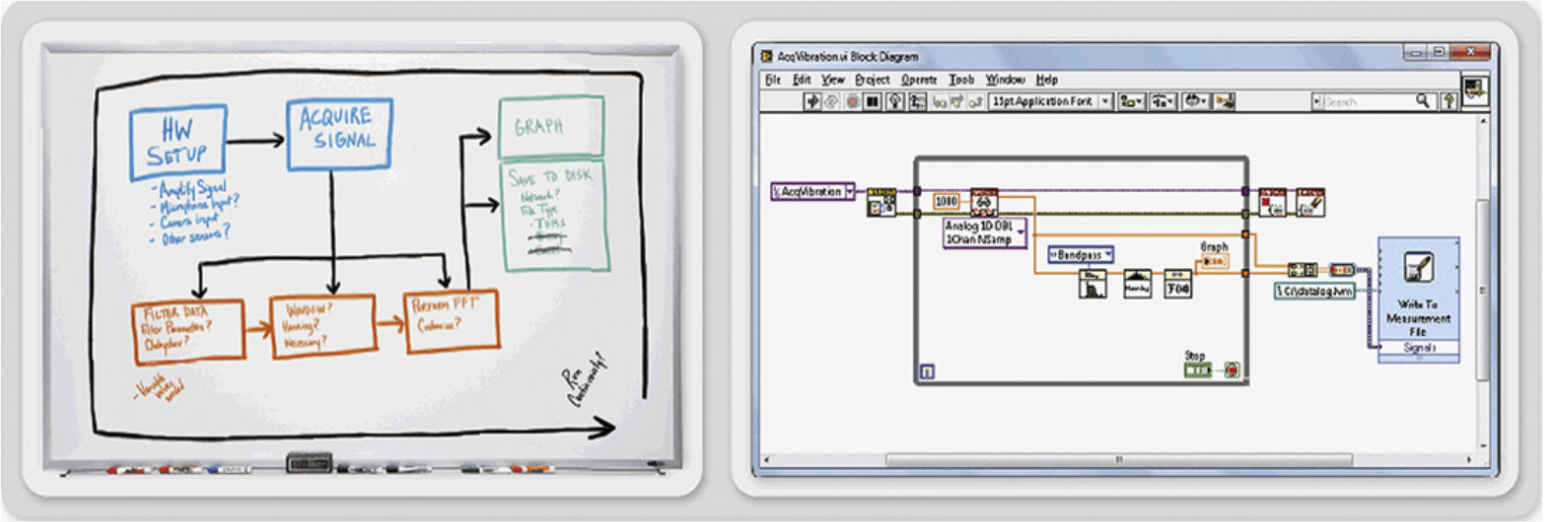
\includegraphics[width=0.9\textwidth]{sketchesVsFormalNotations.png}
    \attribution{N. Medvidovic}
\end{center}

Самые ходовые модели, на самом деле, неформальные. Большая часть полезных моделей служит только для поддержки общения, такие модели рисуются на доске, их обсуждают и тут же стирают, в лучшем случае фотографируя. Более формальные модели используются в документации, там их некому вживую пояснить, поэтому требуется использовать более-менее стандартные языки моделирования (например, UML) --- чтобы даже если систему отдали на аутсорсинг в Индию, архитектуру поняли бы однозначно. Самые формальные модели --- исполнимые, это полноценные языки программирования, только в графическом синтаксисе (например, LabVIEW, модель на картинке, справа --- на нём по-настоящему программируются микроконтроллеры и даже целые их сети).

Рассмотрим, какого рода модели вообще используются при проектировании программного обеспечения.

\subsubsection{Естественный язык}

Самый распространённый вид моделей, который обычно даже моделями-то не считается --- это просто текст на естественном языке. Вот простой пример текстовой модели игры <<Посадка на луну>> из лекции проф. N. Medvidovic:

\begin{center}
    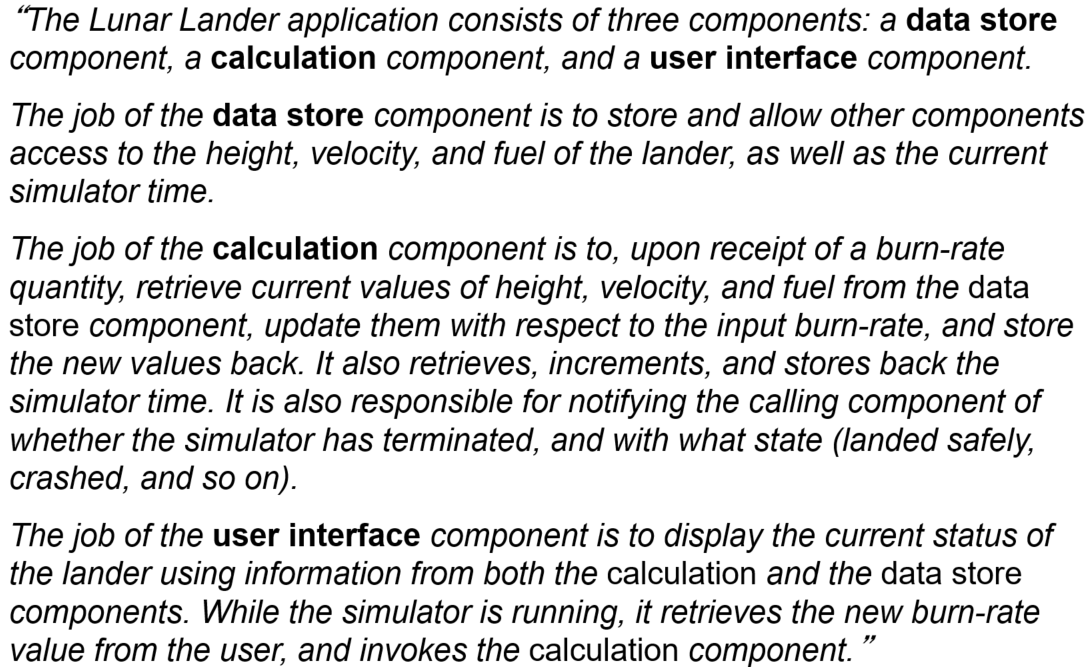
\includegraphics[width=0.6\textwidth]{naturalLanguage.png}
    \attribution{N. Medvidovic}
\end{center}

Преимущества моделей на естественном языке очевидны --- чтобы читать такие модели, не требуется учить синтаксис новых языков, язык очень выразителен (в буквальном смысле позволяет описать все мыслимые модели), максимально гибок. Недостатки, впрочем, тоже очевидны --- естественный язык неформален, не строг, слишком многословен, бесполезен для автоматической обработки (в этом плане последние достижения в NLP дают некоторую надежду, но пока что алгоритмы разбора текстов на естественных языках очень далеки от применения в инструментах разработки архитектуры).

\subsubsection{Неформальные графические модели}

Активно используются и неформальные графические модели --- диаграммы, рисуемые в PowerPoint, InkScape, Visio (без плагина UML) и подобных редакторах. На самом деле, такие диаграммы, скорее всего, встречаются в мире разработки ПО даже чаще, чем UML-диаграммы:

\begin{center}
    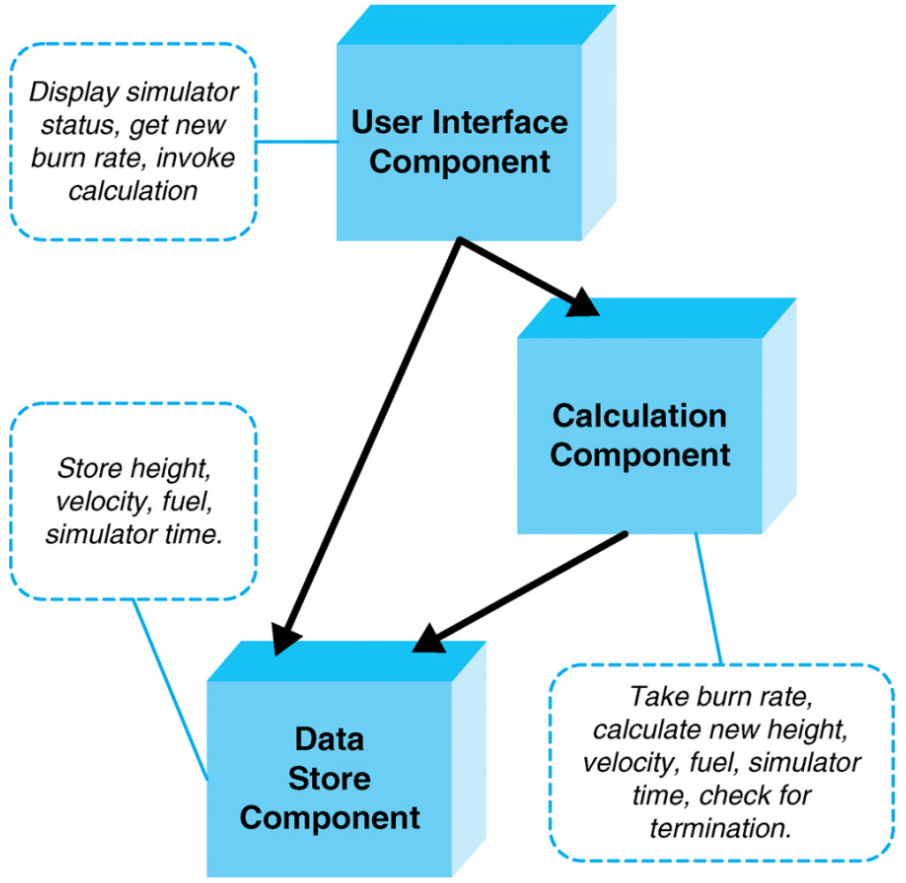
\includegraphics[width=0.4\textwidth]{informalModel.png}
    \attribution{N. Medvidovic}
\end{center}

Преимущества такого подхода --- простота понимания (опять-таки, не требуют специальных знаний), очень гибкая нотация, их можно сделать чисто внешне красивыми. Недостатки --- опять-таки неформальность, нестрогость и неоднозначность, и тут, в отличие от текстовых моделей, есть подводный камень --- неформальные диаграммы часто воспринимаются неспециалистами как формальные и строгие. Такие диаграммы всё ещё практически бесполезны для автоматической обработки. Фигуры и линии с их координатами обычно несложно достать из файлов сохранения, но потом их приходится мучительно парсить, чтобы программно понять смысл нарисованного. Например, в Visio фигура и текст, который внутри написан, могут быть формально никак не связаны и даже храниться в разных частях файла.

\subsubsection{Формальные графические модели}

Формальные графические модели --- это прежде всего модели на формальных языках типа UML, SysML, Entity-Relationship, IDEF0 и т.д., таких языков довольно много. Такие языки часто состоят из нескольких разных нотаций (или <<диаграмм>>), позволяющих отдельно моделировать разные точки зрения на систему, стандартны --- в чём их главное преимущество перед способами, рассмотренными выше --- и, поэтому, имеют хорошую инструментальную поддержку (например, существует больше десятка только популярных UML-инструментов для создания архитектурных моделей, непопулярных тысячи). Важным достоинством является формальность языков, что может быть непривычно для людей, привыкших воспринимать UML как картинки --- у UML и у любого другого такого языка есть строгий синтаксис, описывающий множество корректных диаграмм, как и у текстовых языков программирования. Важный недостаток формальных графических моделей --- частое отсутствие строгой семантики (в UML из 14 видов диаграмм формальная семантика хоть как-то описана только для двух, хотя синтаксис подробно описан для каждой). Кроме того, поскольку такие языки поддерживают много точек зрения, между ними сложно обеспечить консистентность, сложно расширять языки и модифицировать их под свои нужды.

Вот пример трёх разных диаграмм (или <<подъязыков>>) UML:

\begin{center}
    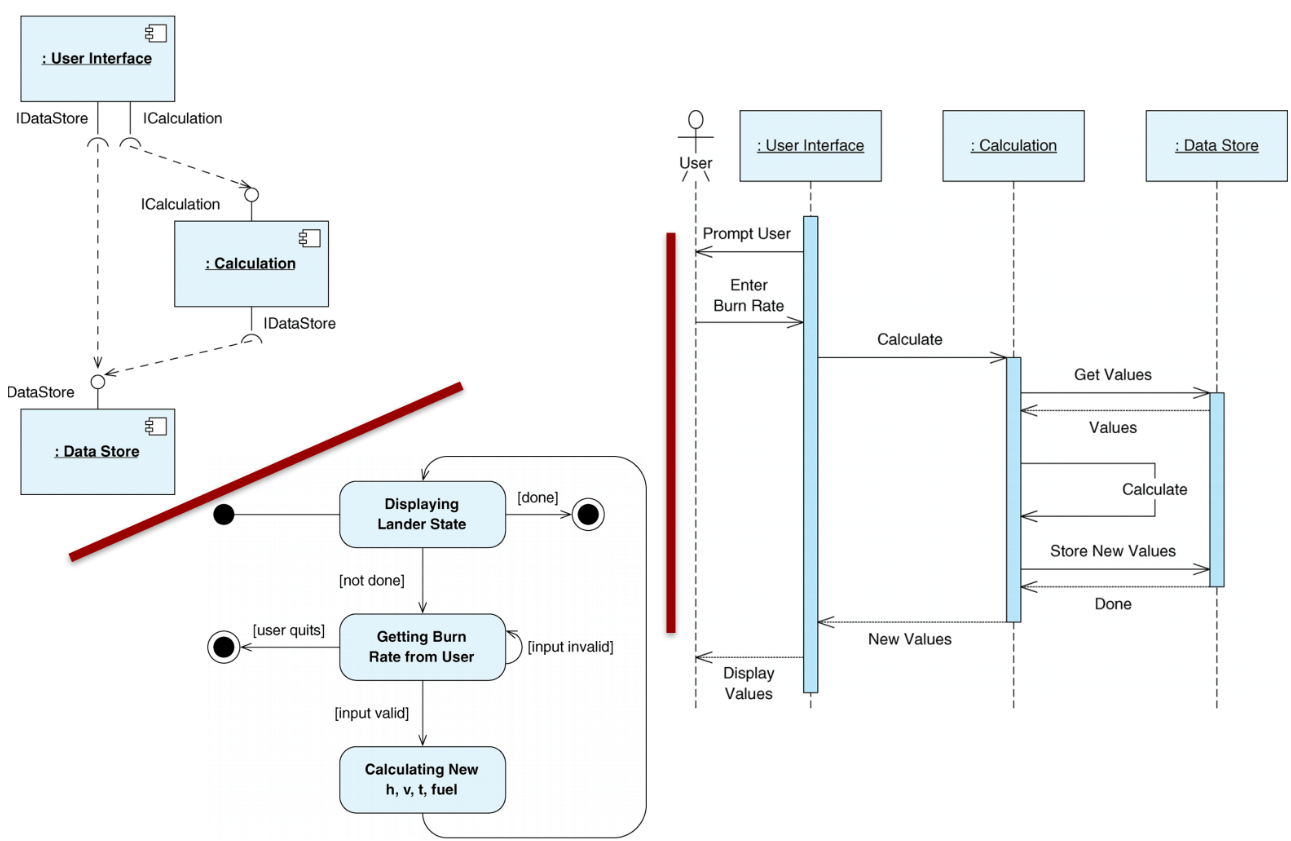
\includegraphics[width=\textwidth]{uml.png}
    \attribution{N. Medvidovic}
\end{center}

\subsubsection{Формальные текстовые языки}

Даже формальные графические языки недостаточно формальны (обычно не имеют исполнимой семантики, что неудивительно, потому что это языки моделирования всё-таки). Поэтому существуют и формальные текстовые языки описания архитектуры, например, AADL (может быть, VHDL можно отнести к таким языкам, хоть он слишком специфичен). Это языки, где компоненты системы и интерфейсы между компонентами описываются формально на языке программирования (но без реализации, конечно), выписываются и доказываются различные утверждения про моделируемую систему (например, ограничения на время отклика, пропускную способность). Пример описания архитектуры на AADL от проф. N. Medvidovic:

\begin{center}
    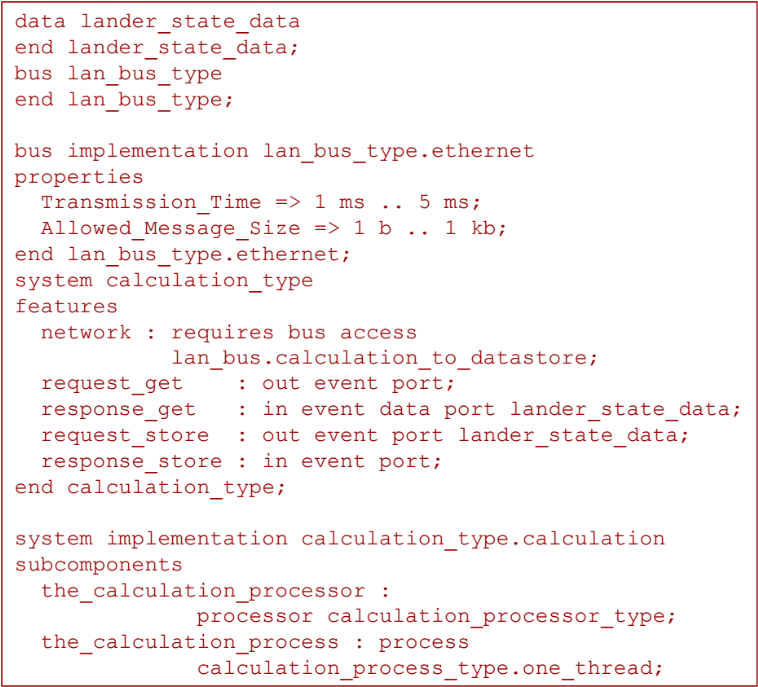
\includegraphics[width=0.65\textwidth]{aadl.png}
    \attribution{N. Medvidovic}
\end{center}

Используются такие языки в основном там, где требуется высокая надёжность и некоторые гарантии на параметры системы --- во встроенных системах, системах реального времени и т.д., они же используются часто при проектировании программно-аппаратных и аппаратных систем.

Основное преимущество подобного подхода --- возможность формального анализа свойств системы ещё до начала реализации, и для AADL существуют весьма продвинутые инструменты анализа. Основные недостатки --- слишком большая многословность и детальность (уже не нарисовать на доске), сложность в изучении и использовании (поэтому в результате одного опроса IT-компаний Турции выяснилось, что половина программистов слыхом не слыхивала про AADL, и я думаю, это типично для IT-сообщества любой страны).

\subsection{Ещё о визуальных моделях}

С архитектурными моделями связано ещё несколько понятий, которые обсуждались в курсе << Разработка программного обеспечения>>, но напомним.

\begin{itemize}
    \item Метафора визуализации --- это договорённость о том, как будут представляться сущности языка. Например, в UML классы представляются в виде прямоугольников, разделённых на три области (имя класса, поля и методы), а в нотации Буча классы представлялись в виде облаков, нарисованных пунктирными линиями (а объекты --- в виде облаков, нарисованных сплошными линиями; ну а что, классы --- это что-то абстрактное). Поскольку программное обеспечение незримо, метафора визуализации --- не более чем договорённость между программистами.
    \item Точка зрения моделирования --- какой аспект системы и для кого моделируется. Наличие такого понятия связано с тем, что модель принципиально проще моделируемой системы, так что приходится выбирать, какие детали оставить за её рамками. Бывают модели для программистов, по которым они должны понять, какие классы и с какими методами надо реализовать, бывают --- для менеджеров, чтобы те могли видеть, сколько уже реализовано и сколько ещё осталось, бывают --- для заказчиков, чтобы объяснить им, что в итоге получится и почему столько стоит. Перед тем, как рисовать диаграмму, важно понять, для кого и зачем мы её рисуем. Не следует рисовать диаграммы просто потому что мы можем.
    \item Семантический разрыв --- принципиальная неспособность модели полностью специфицировать систему; разрыв между информацией, содержащейся в модели и информацией, необходимой, чтобы компьютер мог выполнить программу, которую эта модель описывает. Впрочем, семантический разрыв --- это не приговор, исполнимые модели бывают и активно используются (впрочем, если быть точными, исполнимая модель --- это не модель, а программа на графическом языке). Чаще всего, однако, в реальной жизни встречаются одноразовые модели --- нужные только для того, чтобы передать идею. Их не то что нельзя исполнить, их часто нельзя даже понять без помощи автора.
\end{itemize}

\section{UML}

Unified Modeling Language (UML) --- пожалуй, самый популярный визуальный язык, используемый для разработки программного обеспечения, стандарт де-факто архитектурного моделирования. Пользуются им далеко не все проекты и компании, но знать его должен каждый уважающий себя программист и, тем более, архитектор, поэтому придётся потерпеть нудное перечисление всех видов диаграмм UML далее. 

UML не любят, в частности, из-за его сложности --- на самом деле это не один язык, а порядка 14 разных языков, объединённых единым стандартом и единым описанием синтаксиса (то есть метамоделью). Обычно когда говорят UML, имеют в виду диаграммы классов, но это только один из 14 языков, бывают совсем другие нотации, описывающие систему с разных точек зрения.

UML разрабатывается консорциумом Object Management Group (OMG), в который входят крупные IT-компании и университеты (более сотни). OMG же стоит за такими стандартами, как CORBA и BPMN. Некоторые версии UML (1.4.2 и 2.4.1, не очень свежие, но good enough) приняты как международные стандарты ISO. Первая из получивших распространение стандартизованная версия UML имела номер сразу 1.1 и появилась в 1997 году, до неё была спецификация 0.9 (1996 год), обратите внимание, примерно в то же время, когда появились первые версии Java. 

Появился UML не из воздуха: компания Rational наняла трёх ведущих методологов, занимавшихся визуальными языками и, собственно, методологией разработки ПО --- Айвара Якобсона, Джеймса Рамбо и Гради Буча (того самого Гради Буча, картинки из знаменитой книжки которого <<Object-oriented analysis and design>> были в предыдущей лекции). Каждый из этих уважаемых людей уже имел свою, и популярную, методологию проектирования. Буч был автором <<метода Буча>> и, кстати, сооснователем компании Rational, Рамбо был автором Object Modeling Technique (откуда в UML пришли диаграммы классов), Якобсон --- автор Object-oriented software engineering, откуда в UML пришли диаграммы случаев использования. Была создана не только единая нотация, призванная покончить с языковой разрозненностью в области архитектуры в начале 90-х, но и единая методология разработки ПО: Rational Unified Process (RUP), бывшая популярной в конце девяностых, но побеждённая Agile-методологиями в начале двухтысячных. RUP предполагал активное использование UML, естественно. И так уж получилось, что компания Rational была первой на рынке с инструментами поддержки UML и RUP (кто бы мог подумать), стала фактическим монополистом в конце 90-х и, наверное, неплохо на этом заработала.

Дальнейшее развитие UML имеет одну серьёзную веху --- UML 2.0 (2005 год), когда язык существенно переработали и приспособили не только для разработки программного обеспечения, но и для аппаратных систем тоже (используется он до сих пор всё-таки в основном программистами, у инженеров и так всё хорошо было с визуальными нотациями и их инструментальной поддержкой). Нотация языка тоже существенно поменялась (например, диаграммы активностей и диаграммы конечных автоматов сделали двумя отдельными языками), так что это иногда приводит к путанице --- в интернетах полно диаграмм в старой нотации. Актуальная на данный момент версия UML --- 2.5.1, принятая в декабре 2017 года.

В UML определён механизм стандартных расширений, даже целых два --- \textit{профили} и \textit{метамоделирование}. Профили --- механизм легковесного расширения, позволяют уточнить уже существующую нотацию UML для использования в какой-то конкретной предметной области. Метамоделирование позволяет взять стандарт UML и его подредактировать, добавив новые элементы или убрав существующие. Это гораздо более трудоёмко, чем профили, и не все инструменты поддерживают такой подход, тогда как профили более-менее широко поддержаны. Тем не менее, и профили, и метамоделирование активно используются самим консорциумом OMG, так что у UML появились языки-<<родственники>> (например, SysML), которые по сути расширения UML через метамоделирование. Есть и куча стандартных профилей UML, но мы не будем в этом курсе на них останавливаться.

\subsection{История UML}

Вот замечательный рисунок из \url{https://modeling-languages.com/history-modeling-languages-one-picture-j-p-tolvanen/}, показывающий взаимосвязь между разными визуальными языками:

\begin{center}
    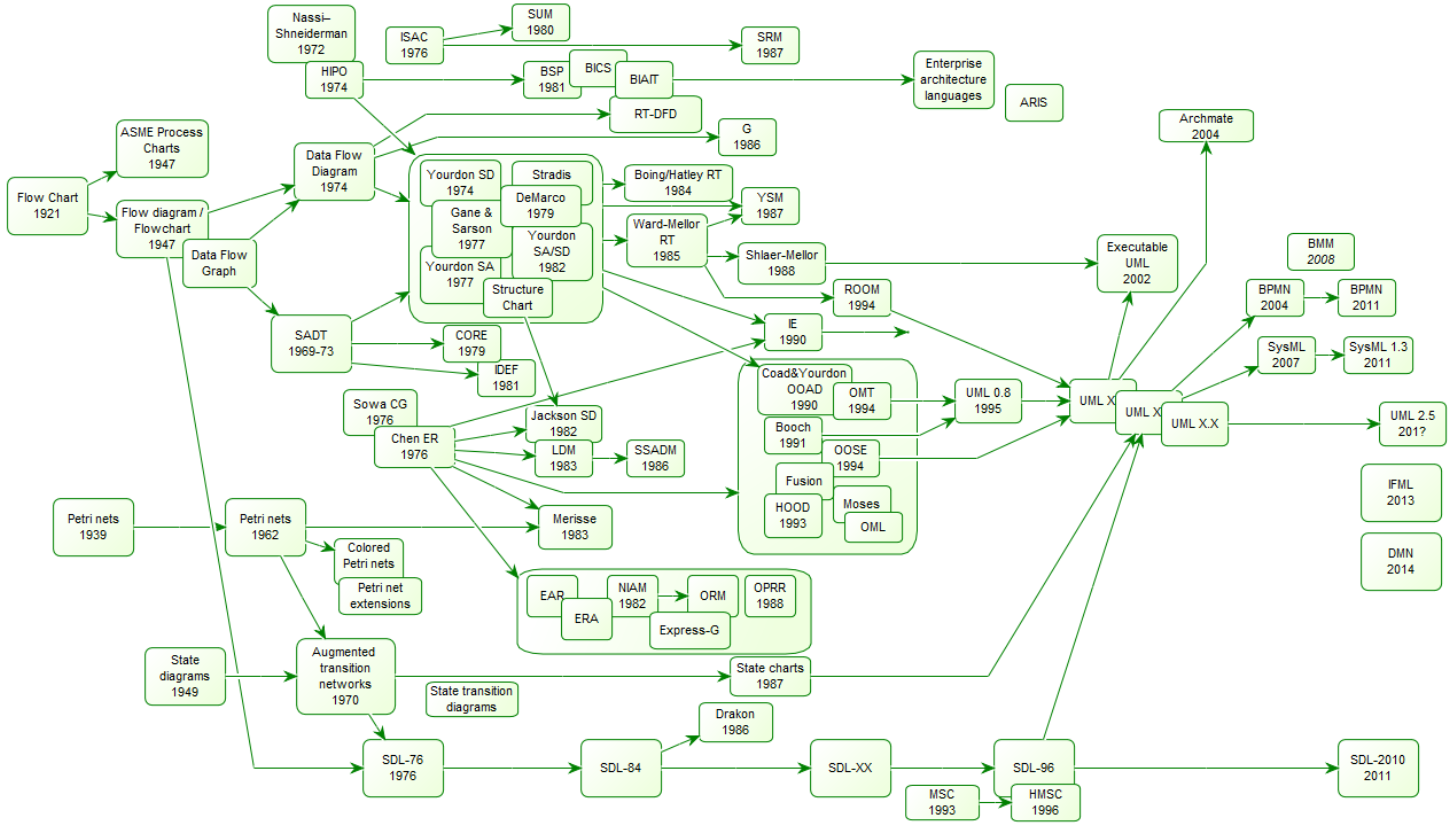
\includegraphics[width=\textwidth]{umlHistory.png}
\end{center}

Как видно из картинки, всё началось ещё до появления электронных компьютеров: различного рода диаграммы использовались давным-давно. Однако серьёзная потребность в моделировании при разработке ПО возникла только в конце 60-х годов, когда уже появились высокоуровневые языки программирования и программы начали становиться сложнее рассчётов по формуле. В это время появляются нотации, которые живы до сих пор: Data Flow Diagram, SADT (Structured Analysis and Design Technique), диаграммы Насси-Шнейдермана (из которых потом появился довольно известный нынче язык Scratch и его идейный продолжатель Google Blockly). На конец 1970-х приходится первый активный всплеск интереса к визуальным языкам и методологиям, появляются нотации SDL (Specification and Description Language), Entity-Relationship, IDEF, все они более чем живы до сих пор (SDL стандарт де-факто при описании телекоммуникационных протоколов, ER --- при проектировании баз данных, семейство языков IDEF применяется в анализе бизнес-процессов). 

Второй пик развития приходится на конец 80-х --- начало 90-х (поиски серебряной пули и языков 4-го поколения, которые повысили бы продуктивность труда программиста так же, как в своё время языки высокого уровня повысили продуктивность по сравнению с ассемблером). Каждая уважающая себя IT-компания считала своим долгом создать свою уникальную технологию на основе визуальных языков, получить огромный прирост производительности (в этом никто особо не преуспел) и ни с кем не поделиться секретом. Тут появляются языки, которые потом лягут в основу UML (нотация Буча, OOSE, OMT), языки, которые войдут в UML как часть, но продолжат развиваться независимо --- SDL, State charts (диаграммы конечных автоматов --- казалось бы, общеизвестная вещь, но формализованы они были Харелом только в 1987 году). Почётного упоминания заслуживает ДРАКОН (Дружественный Русский Алгоритмический язык, Который Обеспечивает Наглядность) Паронджанова, язык G, который до сих пор используется в LabVIEW и средах на её основе --- Robolab и, внезапно, стандартной среде для программирования роботов Lego. Андрей Николаевич Терехов создавал редакторы SDL и технологию RTST примерно в это же время.

В 1995 году появляются первые нестандартизованные спецификации UML, которые оканчивают эпоху языкового зоопарка, дальше UML плавно развивается до версии 2.0, которая вышла в 2005 году, это дало толчок к развитию кучи профилей UML или языков, родственных UML --- Executable UML, BPMN, SysML и т.д. Параллельно развивались языки описания архитектур предприятий, и также в начале-середине двухтысячных стали модны предметно-ориентированные визуальные языки. Однако постепенно интерес к визуальным языкам пошёл на спад. Отчасти это произошло из-за Agile Manifesto, где было написано, что документация --- это хорошо, но работающий код лучше; диаграммы не являются работающим кодом, семантический разрыв и всё такое. Отчасти --- из-за того, что визуальные языки так и не показали обещанного прироста продуктивности, хайп угас и стало понятно, что визуальные языки --- это сложно, очень тяжело в инструментальной поддержке и, в общем-то, не очень нужно. Тем не менее, UML всё ещё активно применяется в индустрии (порядка половины компаний-разработчиков его так или иначе используют), другие визуальные языки тоже сохранили свои экологические ниши и нынче хайп имеет шансы вернуться с новой силой в контексте end-user programming, интернета вещей и т.п.

\subsection{Диаграммы UML}

Перейдём, собственно, к UML. Как вы, наверное, помните, UML 2.5.1 состоит из 14 видов диаграмм, довольно слабо связанных друг с другом, вот картинка (из UML Specification), где все эти диаграммы перечислены:

\begin{center}
    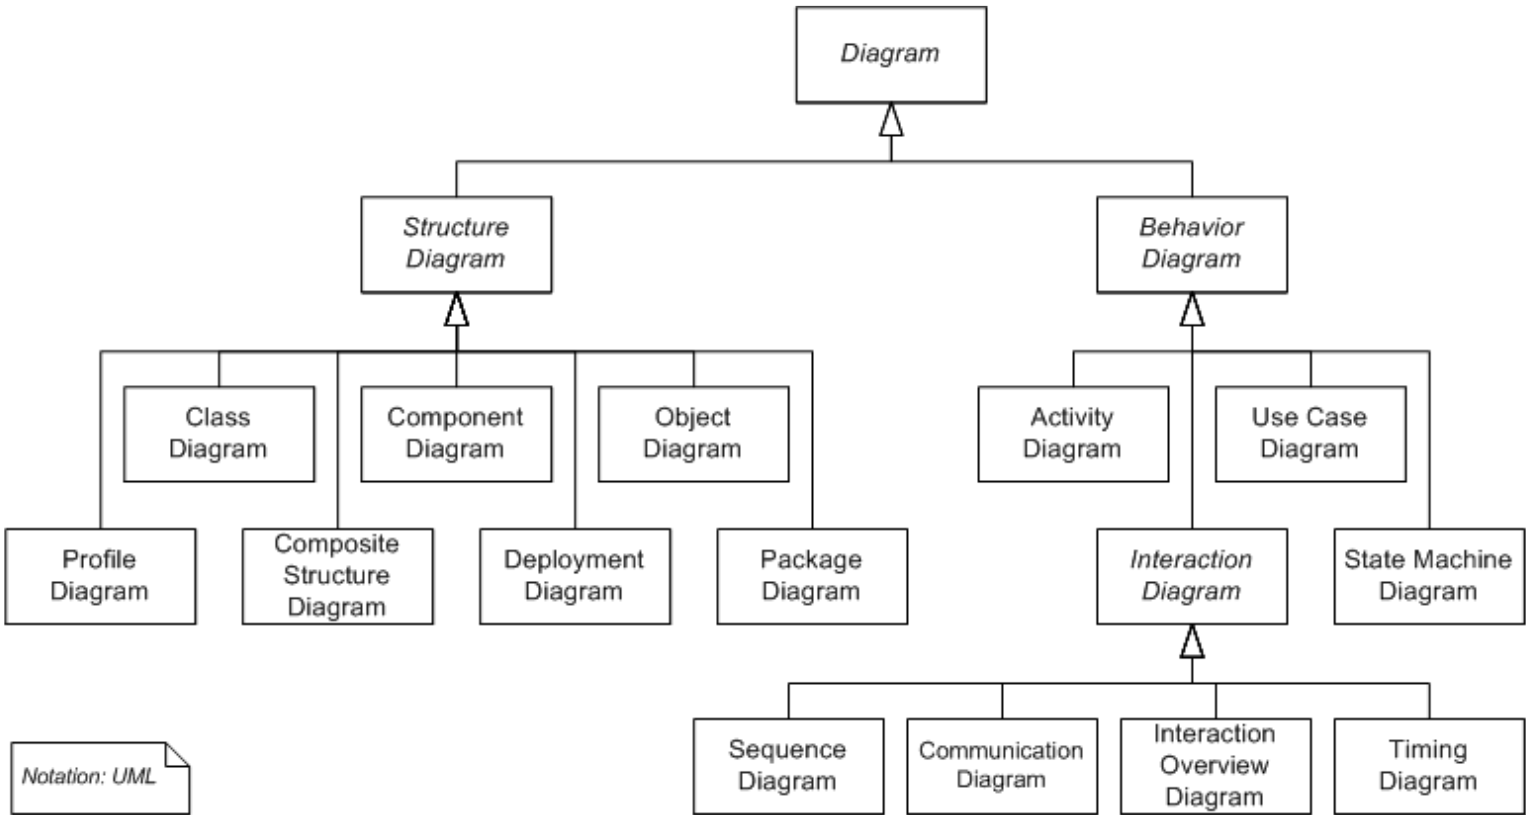
\includegraphics[width=\textwidth]{umlDiagrams.png}
\end{center}

Сама картинка --- это диаграмма классов UML, кстати.

Диаграммы делятся на две крупные категории --- структурные и поведенческие. Структурные диаграммы показывают структуру системы времени компиляции --- это прежде всего диаграмма классов, диаграмма компонентов, диаграмма пакетов и другие. Поведенческие диаграммы показывают, как система себя ведёт во время работы --- это диаграммы состояний, диаграммы последовательностей, диаграммы активностей, сюда же относят диаграммы случаев использования и другие, более специализированные диаграммы.

\section{Диаграммы классов UML}

\subsection{Диаграмма классов, общий синтаксис}

Самая известная диаграмма UML --- это, пожалуй, диаграмма классов. Её внешний вид и описание элементов из книжки М. Фаулера <<UML. Основы>> (кстати, книга очень рекомендуется как быстрая справка по UML, информации в которой вполне достаточно, чтобы успешно пользоваться языком):

\begin{center}
    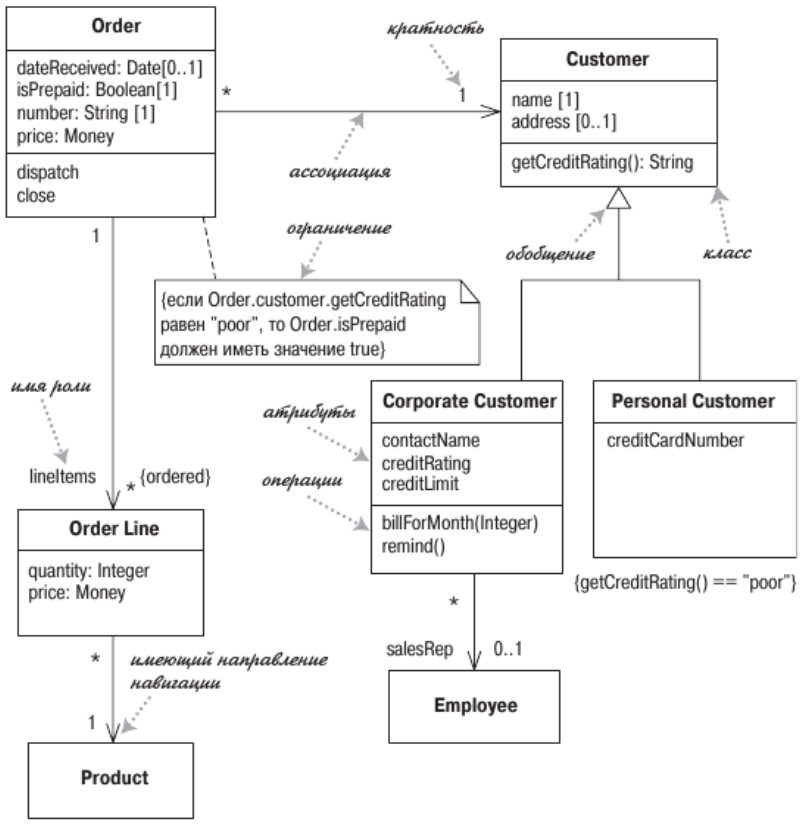
\includegraphics[width=0.8\textwidth]{umlClassDiagram.png}
    \attribution{М. Фаулер. <<UML. Основы>>}
\end{center}

В общем-то, пояснений картинка не требует, надо только обратить внимание, что наследование в UML называется <<обобщение>> (generalization) и стрелка указывает на предка, а не на потомка (с этим часто путаются). Кратность ассоциации тоже может вызвать путаницу, она пишется у того конца ассоциации, к которому относится кратность. Например, Customer может иметь много Order (звёздочка означает <<0 или больше>>), но у каждого Order ровно один Customer. 

Ещё одна важная особенность всех UML-диаграмм --- это то, что они допускают не отображать некоторую информацию, если автор считает её не важной в данном контексте (вспомните про точку зрения моделирования). Например, на рисунке выше неверно, что класс Employee не имеет ни методов, ни полей, просто автор посчитал, что они не важны и решил не загромождать диаграмму. То же касается и ассоциаций --- отсутствие множественностей или стрелок означает лишь, что они не специфицированы, они вполне могут быть выбраны самостоятельно программистом, который реализует систему.

\subsection{Как это связано с кодом}

Как диаграммы классов связаны с кодом, лучше всего пояснить на примере. Если у нас есть такая диаграмма классов:

\begin{center}
    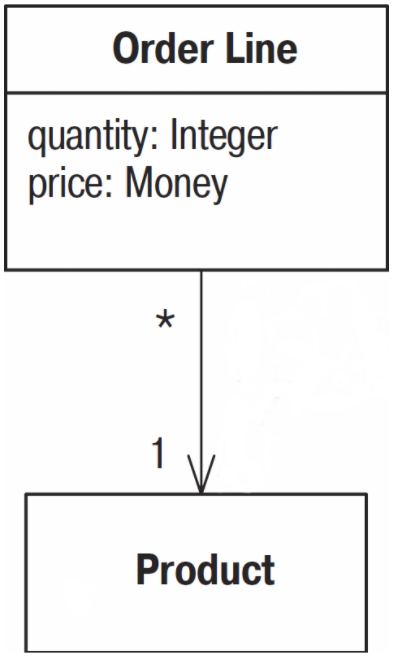
\includegraphics[width=0.2\textwidth]{orderLine.png}
\end{center}

то по ней можно написать (или сгенерировать, по крайней мере большую часть) вот такой код (для примера, на Java):

\begin{minted}{java}
public class OrderLine {
    private int quantity;
    private Product product;

    public int getQuantity() {
        return quantity;
    }

    public void setQuantity(int quantity) {
        this.quantity = quantity;
    }

    public Money getPrice() {
        return product.getPrice().multiply(quantity);
    }
}
\end{minted}

Класс Product тут для краткости не показан, благо на диаграмме про него всё равно никаких подробностей не приводится. Обратите внимание, что навигабельная ассоциация стала полем, а поле price в ходе реализации превратилось не в поле, а в вычислимое свойство. Такие преобразования тоже вполне допустимы, если программист-реализатор считает, что так удобнее (хотя для вычислимых свойств в UML есть отдельная нотация, <</>> перед именем свойства).

С двунаправленными ассоциациями несколько хитрее, потому что при реализации требуется ещё некий механизм поддержания целостности обоих концов ассоциации. Например, диаграмма

\begin{center}
    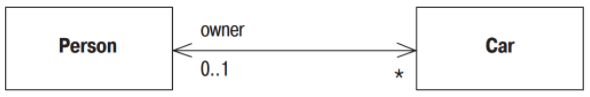
\includegraphics[width=0.5\textwidth]{twoWayAssociations.png}
\end{center}

могла бы быть реализована следующим образом (теперь на C\#, для разнообразия):

\begin{minted}{csharp}
class Car {
    public Person Owner {
        get { return _owner; }
        set {
            if (_owner != null) 
            {
                _owner.friendCars().Remove(this);
            }

            _owner = value;
            if (_owner != null) 
            {
                _owner.friendCars().Add(this);
            }
        }
    }
    private Person _owner;
}

class Person {
    public IList Cars {
        get { return ArrayList.ReadOnly(_cars); }
    }

    public void AddCar(Car arg) {
        arg.Owner = this;
    }

    private IList _cars = new ArrayList();

    internal IList friendCars() {
        // должен быть использован только Car.Owner
        return _cars;
    }
}
\end{minted}

В C\# нет аналога ключевому слову friend из C++, так что приходится использовать метод с пакетной видимостью, чтобы ограничить его использование. Но общий смысл тут такой, что при изменении одного конца ассоциации надо не забыть поменять и объект на другом конце --- сказать ему, что мы что-то добавили или что-то удалили.

\subsection{Агрегация и композиция}

Агрегация и композиция ---- дальнейшие уточнения ассоциации. На самом деле, если на диаграмме нарисована просто ассоциация, то при реализации мы вправе выбрать, агрегацию или композицию использовать. Разница между агрегацией и композицией --- во владении объектами, которые участвуют в ассоциации. Агрегация не предполагает владения:

\begin{center}
    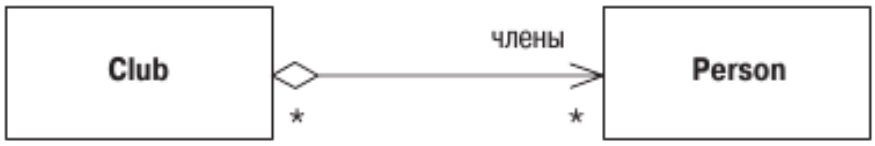
\includegraphics[width=0.5\textwidth]{aggregation.png}
\end{center}

Человек и клуб могут существовать независимо друг от друга, и когда закрывается клуб, его члены продолжают существовать (если это не тоталитарная секта). На диаграмме выше нарисовано, что в клубе может состоять несколько человек, и человек может состоять в нескольких клубах, при этом клуб знает о человеке, но не владеет им.

Композиция говорит, что один объект владеет другим объектом, то есть время их жизни связано и <<хозяин>> отвечает за удаление подчинённого ему объекта. Например, если мы пишем графический редактор, вполне может быть, что мы сделаем так:

\begin{center}
    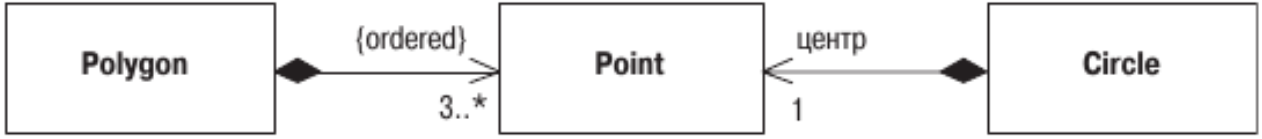
\includegraphics[width=0.7\textwidth]{composition.png}
\end{center}

Здесь многоугольник состоит из точек, и когда мы удаляем многоугольник, удаляются и все точки, которые его определяют. Круг тоже имеет одну точку --- центр круга, и тоже, удаляем круг --- удаляется и его центр. Так что и круг и многоугольник владеют своими точками, но у каждой точки во время исполнения может быть только один хозяин.

Агрегация и композиция важны, если в итоге мы будем писать на C++, там они помогают следить за тем, кто в итоге должен освободить память из-под объекта. Для языков со сборкой мусора это не так важно (хотя и полезно знать, кто кем владеет), поэтому агрегация с композицией используются в диаграммах классов довольно редко --- обычно архитекторы ограничиваются ассоциациями, не специфицируя, агрегация эта конкретная ассоциация или композиция.

С точки зрения нотации надо запомнить, что агрегация --- более слабое отношение, чем композиция, поэтому и ромбик в случае агрегации не закрашен. И ромбики рисуются около контейнера (то есть клуб содержит людей, а не наоборот) --- можно понимать ромбик как оперение стрелы, указывающей от контейнера к содержащемуся в нём объекту. Ещё один небольшой пример:

\begin{center}
    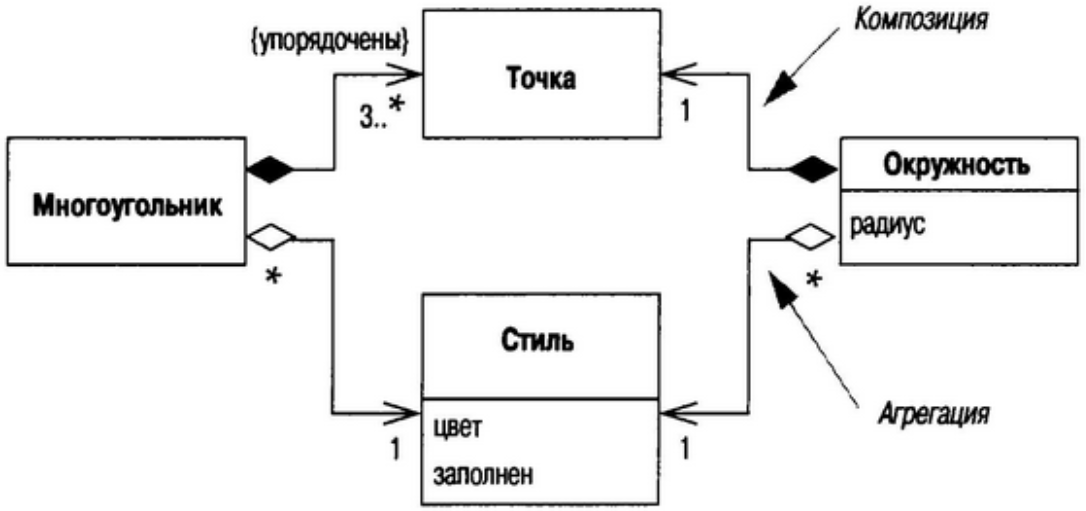
\includegraphics[width=0.6\textwidth]{aggregationAndCompositionExample.png}
    \attribution{М. Фаулер. <<UML. Основы>>}
\end{center}

Многоугольник и окружность владеют своими точками, но не владеют стилями --- у каждой геометрической фигуры должен быть стиль, но стили существуют независимо и могут переиспользоваться между фигурами. Точки между фигурами переиспользованы быть не могут.

\section{Диаграммы пакетов}

Диаграммы пакетов --- это тоже структурные диаграммы, нужны они для того, чтобы показать разбиение кода по пакетам, либо сгруппировать по пакетам саму модель. <<Пакет>> в UML означает более-менее то же, что пакет в Java или пространство имён в C++. Синтаксис диаграммы пакетов очень простой:

\begin{center}
    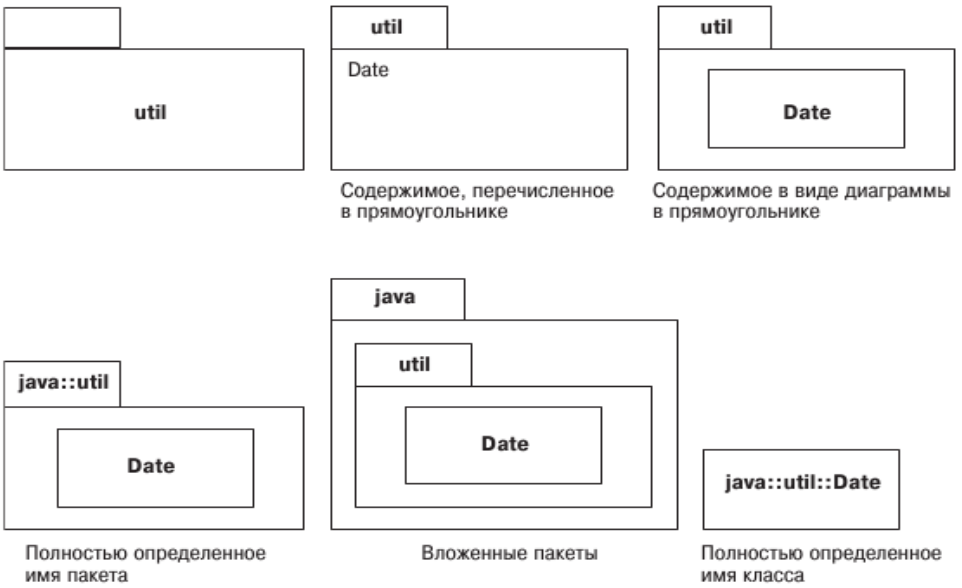
\includegraphics[width=0.8\textwidth]{packageDiagrams.png}
    \attribution{М. Фаулер. <<UML. Основы>>}
\end{center}

На диаграммах пакетов также могут рисоваться компоненты и классы, которые в этих пакетах находятся. Это ещё одна не вполне очевидная особенность UML --- диаграммы не являются отдельными языками, более того, в спецификации UML разбиения на диаграммы нет. Язык описывается единой метамоделью (сгруппированной по пакетам, кстати), а какие элементы на каких диаграммах рекомендуется рисовать, описано только в приложении к стандарту. Так что теоретически всё что угодно можно рисовать где угодно, хотя правила здравого смысла иногда этому мешают. Например, рисовать сущности структурных и поведенческих диаграмм на одной диаграмме нельзя, потому что это может сильно запутать читателя.

\section{Диаграммы объектов}

Диаграммы объектов визуализируют объекты в памяти во время работы программы и отношения между ними (так что по смыслу относятся к поведенческим диаграммам, но все их всё равно считают структурными, поскольку они описывают структуру времени выполнения, а не характер взаимодействия объектов). Диаграммы объектов можно понимать как снимок в какой-то определённый момент времени состояния системы, при этом множество всех возможных состояний описывается диаграммой классов.

Диаграммы объектов используют в двух случаях:

\begin{itemize}
    \item чтобы визуализировать и проиллюстрировать диаграммы классов (как на рисунке ниже, по диаграмме классов не сразу очевидно, что она описывает дерево, а по диаграмме объектов --- сразу);
    \item чтобы разобраться во взаимосвязях реально существующих объектов предметной области, ещё до того, как создана первая диаграмма классов (и тогда диаграмма классов будет на самом деле наведением классификации на объекты, выделенные на диаграмме объектов). Обращаю внимание на этот случай использования, мы увидим примеры применения диаграмм объектов в качестве инструмента анализа предметной области, когда дойдём до методологии предметно-ориентированного проектирования.
\end{itemize}

Синтаксис диаграмм объектов показан на этом рисунке:

\begin{center}
    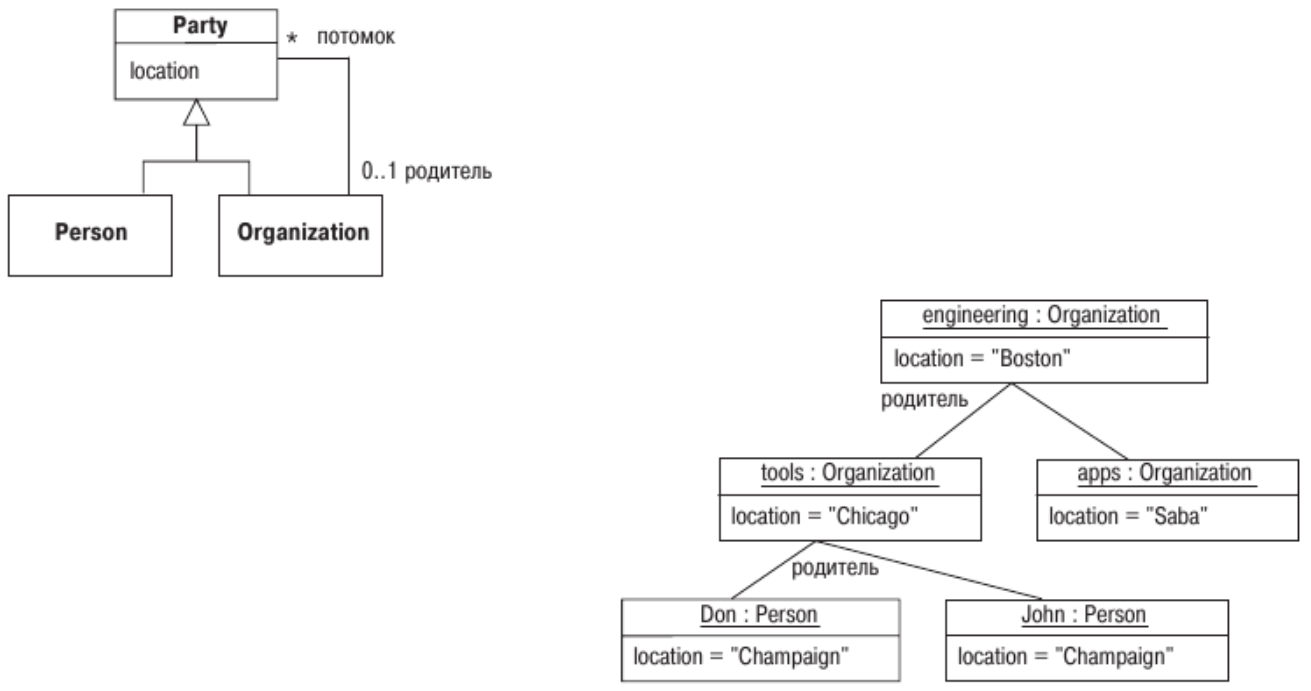
\includegraphics[width=0.9\textwidth]{objectDiagrams.png}
    \attribution{М. Фаулер. <<UML. Основы>>}
\end{center}

Объект рисуется как класс, только его имя подчёркивается, указывается его тип, и каждому атрибуту ставится в соответствие значение.

\section{Диаграммы компонентов}

Диаграммы компонентов --- пожалуй, самые полезные для архитектора диаграммы UML. На них изображаются компоненты, из которых состоит система или подсистема, и взаимосвязи между ними. Точного определения термина <<компонент>> не существует, но все интуитивно представляют, что это такое --- нечто структурно связанное и больше, чем класс. Компонентами могут быть пакеты, пространства имён, сборки, .dll/.so-файлы, отдельные веб-сервисы в распределённом приложении и т.д. В общем, это именно то, из чего состоит высокоуровневая архитектура приложения.

Почему диаграммы компонентов важнее и полезнее диаграмм классов --- они переживают большую часть рефакторингов. Диаграммы классов придётся перерисовывать каждый раз, когда кто-то поменял название какого-нибудь класса или даже метода, добавил поле и т.д. Диаграммы компонентов неизменны до глобальной переработки архитектуры, которая в типичных проектах происходит только раз в несколько лет, так что у диаграмм компонентов много шансов сохранить свою актуальность в долгосрочной перспективе.

Полезны диаграммы компонентов как вид <<с высоты птичьего полёта>> на создаваемую систему. Например, вот диаграмма, описывающая высокоуровневую архитектуру проекта QReal (\url{https://github.com/qreal/qreal}, инструмент для создания визуальных предметно-ориентированных языков и работы с ними):

\begin{center}
    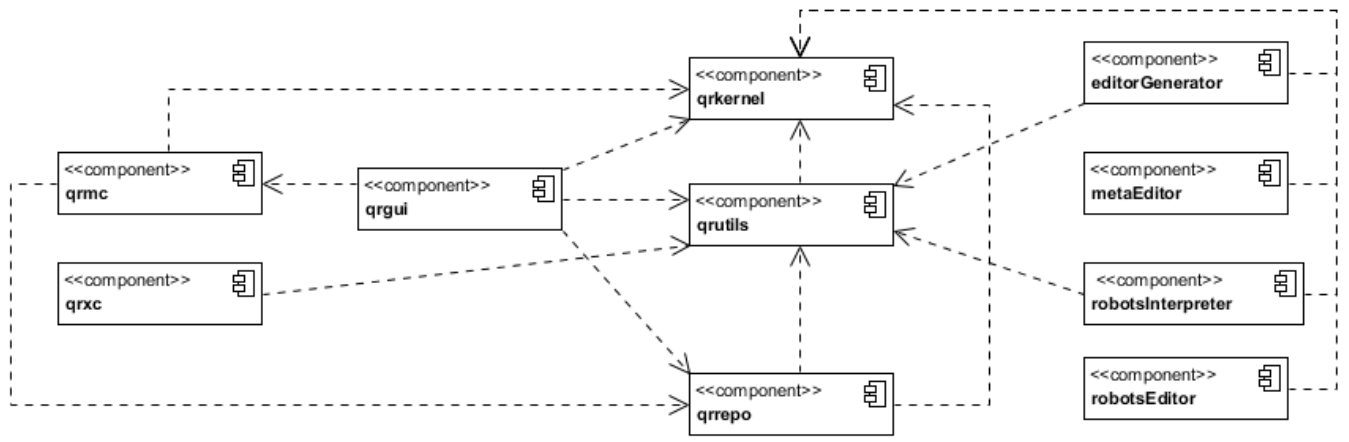
\includegraphics[width=0.95\textwidth]{componentDiagrams.png}
\end{center}

Связи между компонентами тут означают зависимости по сборке, каждый компонент --- это отдельный проект, который собирается в отдельный .dll/.so-файл. По такой диаграмме можно очень быстро рассказать общую архитектуру проекта: qrkernel ни от кого не зависит, там находятся классы, общие для всей системы; qrutils содержит полезную функциональность, используемую в других модулях; qrrepo --- репозиторий, где хранятся данные, с которыми QReal работает; qrgui --- пользовательский интерфейс; qrmc и qrxc --- это компиляторы визуальных языков, с которыми работает QReal; editorGenerator, metaEditor, robotsInterpreter, robotsEditor --- это плагины инструментальной поддержки работы с визуальными языками. Конечно, это не полноценное архитектурное описание, но даже этого достаточно, чтобы было понятно, куда смотреть в исходниках.

Вот описание синтаксиса диаграмм компонентов, на сей раз с сайта \url{http://www.uml-diagrams.org} (очень рекомендую, как быструю справку по синтаксису и как набор примеров с пояснениями):

\begin{center}
    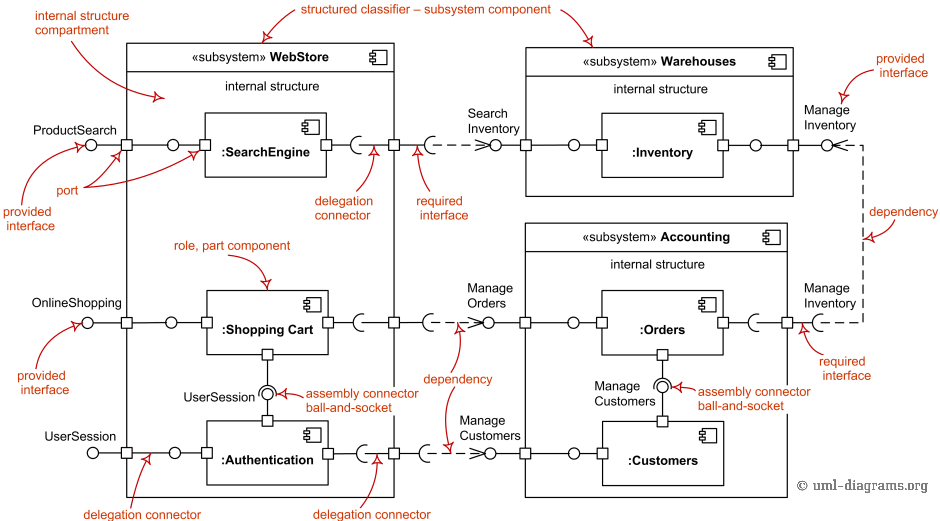
\includegraphics[width=0.95\textwidth]{componentDiagramsOverview.png}
    \attribution{\url{http://www.uml-diagrams.org}}
\end{center}

Видно, что компоненты могут быть вложенными друг в друга, что они могут иметь интерфейсы (так же, как и классы, но на диаграммах компонентов чаще всего используется только <<леденцовая>> нотация). У компонентов есть порты, которые могут предоставлять или потреблять интерфейсы, но порты часто не рисуются, а подразумеваются, поскольку обычно порт имеет только один интерфейс. Порты бывают полезны для изображения делегирования --- что компонент просто перенаправляет запросы вложенному компоненту. Слова \verb|<<subsystem>>| и \verb|<<internal structure>>| опциональны (и обычно не пишутся).

\section{Диаграмма случаев использования UML}

Диаграммы случаев использования UML (также известные как диаграммы прецедентов, use case-диаграммы) появились до UML, как часть методологии OOSE, разработанной Айваром Якобсоном в 1992 году. OOSE на самом деле строилась вокруг случаев использования, их предлагалось продумать первыми, затем на их базе уже проектировать остальную архитектуру, непрерывно поддерживая связь со случаями использования (чтобы не делать лишней работы и быть уверенными, что вся требуемая функциональность где-то реализована). Потом Якобсон перешёл на работу в Rational и стал одним из трёх основателей UML, диаграммы случаев использования попали в язык практически без изменений.

Диаграммы очень простые, состоят всего из двух типов сущностей и границы системы:

\begin{center}
    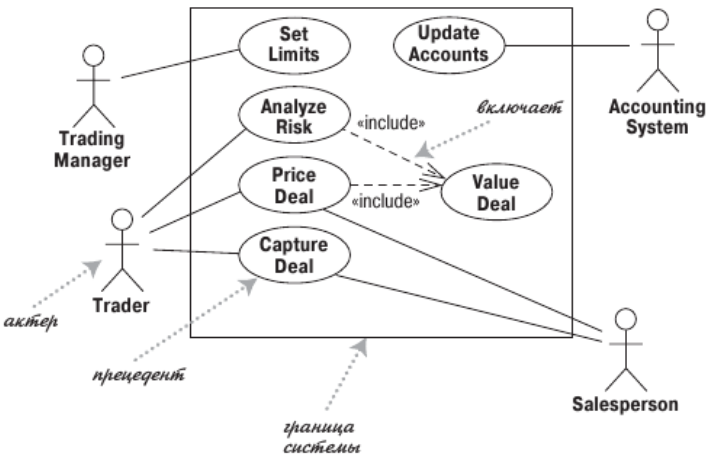
\includegraphics[width=0.6\textwidth]{useCaseDiagram.png}
    \attribution{М. Фаулер, UML. Основы}
\end{center}

\begin{itemize}
    \item Акторы (или актёры, роли, это всё неудачные переводы со шведского на английский и с английского на русский) --- внешние сущности, использующие систему. Это могут быть группы пользователей, объединённые общей целью использования системы (роли, собственно). Это могут быть также внешние программные системы, которые пользуются нашей. Иногда в качестве акторов рисуются и другие программные системы (или люди), которые нужны нашей системе для работы, но это неканонично и лучше так не делать, чтобы не путать читателей.
    \item Случаи использования (прецеденты)  --- цель использования системы актором. Это одно-два-три слова, описывающие, что пользователь хочет в итоге получить (например, <<Проанализировать риски>>, <<Оценить сделку>>). Их часто путают с функциональностью системы, например, <<Залогиниться>> --- это не то же самое. Пользователь никогда не имеет целью использования системы залогиниться, в лучшем случае он хочет безопасного выполнения всех операций, но нефункциональные требования --- это тоже не случаи использования, так что на этой диаграмме не рисуются.

    Случаи использования формулируются слишком кратко, чтобы быть полезными сами по себе, поэтому каждый случай использования должен раскрываться в один или несколько \textit{сценариев использования} системы. Сценарии использования как раз и говорят, что и в каком порядке делает пользователь, чтобы достичь цели (например, логинится -> выбирает нужную сделку -> анализирует риски -> записывает результаты анализа в соответствующую форму). Сценарии чаще всего описываются просто текстом, часто неформальным, иногда как-то структурированным (например, user story из Scrum). Если вы очень любите визуальное моделирование, сценарии использования можно описывать диаграммами активностей UML.
\end{itemize}

\subsection{Сценарии использования}

Каждый случай использования раскрывается в один или несколько сценариев использования. Иногда используются формальные описания сценариев использования, рассмотрим их, чтобы понимать, что вообще там надо писать.

Типичная структура сценария использования такова.

\begin{itemize}
    \item Заголовок --- цель основного актора, собственно, случай использования.
    \item Заинтересованные лица, акторы, основной актор --- сюда выписываются все роли, участвующие в сценарии, среди них выделяется одна --- которая инициирует исполнение сценария.
    \item Предусловия --- какие логические условия должны быть истинны, чтобы сценарий в принципе мог быть исполнен.
    \item Триггеры (активаторы) --- что должно произойти, чтобы сценарий начал выполняться, при условии, что все предусловия выполнены.
    \item Основной порядок событий --- что происходит, если всё идёт по плану. Сюда пишется наиболее типичная последовательность действий.
    \item Альтернативные пути и расширения --- сюда пишется, что делать в нетипичной ситуации, тут же описываются точки расширения и реакция на ошибки.
    \item Постусловия --- какие логические условия должны быть истинны после исполнения сценария.
\end{itemize}

Вот пример карточки сценария использования, сделанной по такой структуре (из книги  R.M. Roth et al., System Analysis and Design):

\begin{center}
    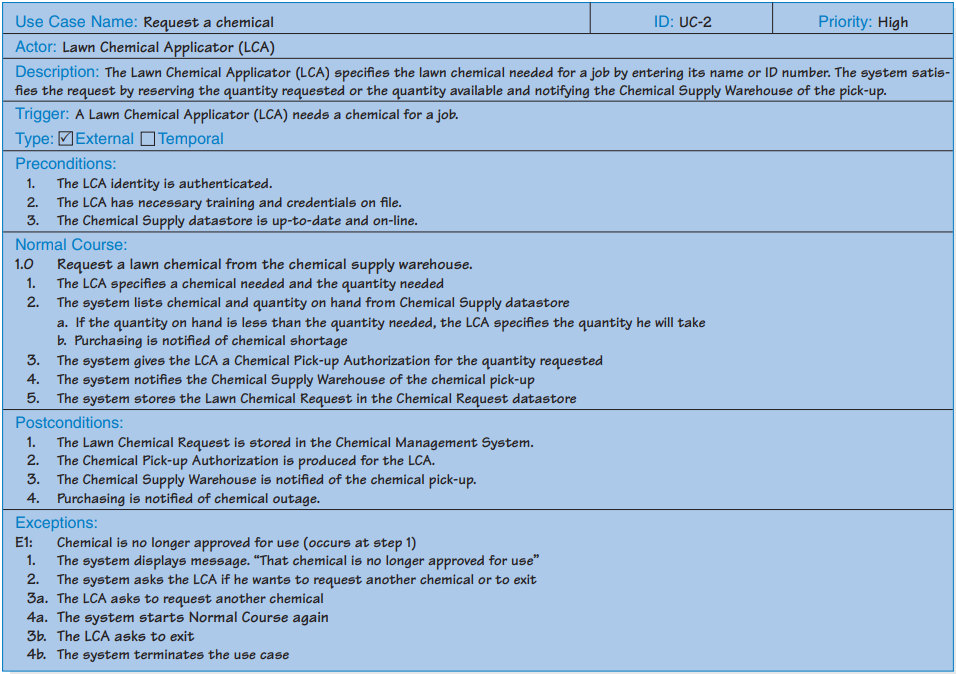
\includegraphics[width=0.95\textwidth]{useCaseExample.png}
    \vspace{3mm}
    \attribution{R.M. Roth et al., System Analysis and Design}
\end{center}

\section{Диаграмма активностей UML}

Важной задачей на этапе анализа, помимо сбора требований, является ещё и анализ бизнес-процессов, которые (или часть которых) мы хотим автоматизировать. Для этого применяются несколько нотаций --- во-первых, диаграммы активностей UML, во-вторых, отдельный язык BPMN (Business Process Model and Notation), который, как и UML, состоит из нескольких видов диаграмм и специально предназначен для моделирования бизнес-процессов.

Диаграммы активностей UML внешне очень напоминают блок-схемы, но используются прежде всего не для моделирования алгоритмов (хотя и для этого тоже, иногда), а для моделирования поведения бизнес-процесса в целом. Кстати, термином <<бизнес-процесс>> в IT принято называть любой процесс работы в организации, может быть, и не связанный с бизнесом. Зачем вообще моделировать процессы --- во-первых, для того, чтобы понять, как в существующий процесс вписывается разрабатываемая система, во-вторых, это хороший способ визуализации сценария использования системы, с точки зрения пользователя.

Кстати, это одна из двух диаграмм UML, для которой описана семантика её исполнения, на основе сетей Петри. Вторая диаграмма --- это диаграмма конечных автоматов, про которую несколько попозже. Выглядит диаграмма активностей (также иногда встречается вариант перевода <<диаграмма деятельностей>>) так:

\begin{center}
    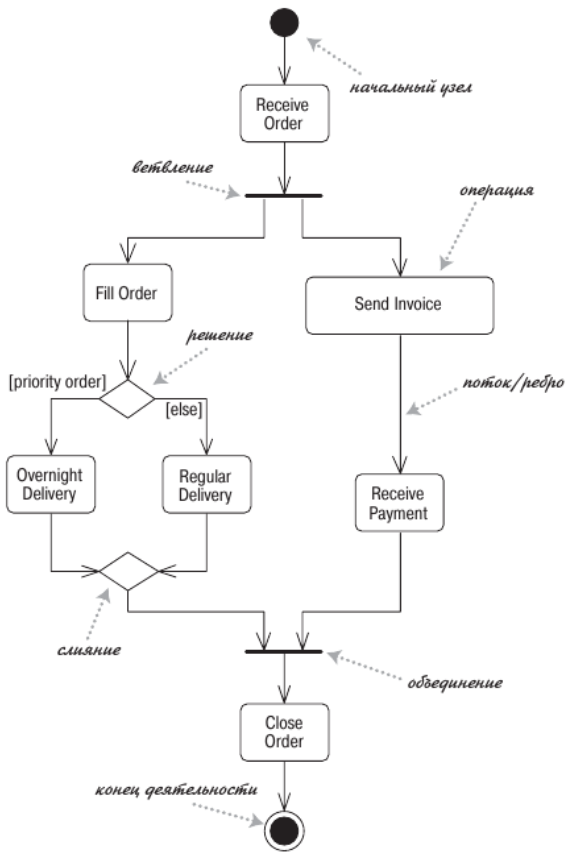
\includegraphics[width=0.5\textwidth]{activityDiagram.png}
    \attribution{М. Фаулер, UML. Основы}
\end{center}

<<Ветвление>>/<<объединение>> работает как fork/join для параллельных потоков --- <<ветвление>> разделяет исполнение на два или больше параллельных потоков, <<объединение>> ждёт, пока все входящие в него потоки закончат исполнение, и только после этого отдаёт управление дальше. Ничто не мешает потоки не объединять, тогда исполнение заканчивается, как только хотя бы один поток дойдёт до блока <<конец деятельности>>. По синтаксису каждый блок <<решение>> может иметь несколько веток (в этом смысле он похож на оператор switch/case в текстовых языках), но все ветки должны сходиться на блоке <<слияние>>. Причём, в отличие от блок-схем, условие пишется не в ромбике, а над каждой исходящей стрелкой, и условия должны быть взаимоисключающими.

\section{Диаграмма развёртывания UML}

Диаграмма развёртывания UML (deployment diagram) используется для того, чтобы показать размещение логических элементов системы (компонентов, исполнимых файлов) на физических или виртуальных устройствах. Пример такой диаграммы:

\begin{center}
    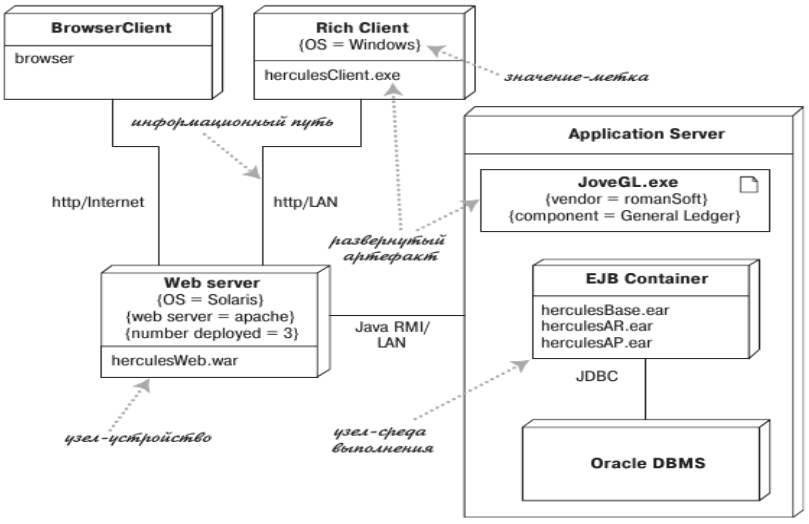
\includegraphics[width=0.7\textwidth]{deploymentDiagram.png}
    \attribution{М. Фаулер, UML. Основы}
\end{center}

Параллелепипедами на диаграмме рисуются устройства или похожие на устройства части системы (реальные компьютеры или группы компьютеров, базы данных, среды выполнения и т.д.). В них рисуются развёрнутые там артефакты (бинарники, компоненты и т.д.). Связи здесь возможны только между узлами (устройствами) и показывают оин физические (или низкоуровневые логические) каналы связи между узлами, с указанием протокола взаимодействия. И узлы, и артефакты могут иметь дополнительные свойства, пишущиеся в фигурных скобках. Артефакты можно рисовать как подробно (прямоугольником), так и кратко (просто надписью с именем артефакта).

Казалось бы, развёртывание происходит ближе к концу разработки, так что не имеет отношения к анализу. Однако оказывается, что часто физические устройства оказываются известны заранее (например, заказчик уже купил два сервера и готов купить ещё пяток терминалов), и наличествующие физические устройства во многом определяют архитектуру системы. Тогда диаграмма развёртывания очень полезна как инструмент именно анализа --- она позволяет отобразить уже существующую инфраструктуру и понять, как мы намерены её использовать.

Ещё одно полезное применение диаграммы развёртывания --- обратное проектирование, когда система у заказчика уже есть, но никто не знает, как она устроена, а вам надо для неё чего-то написать. Как правило, даже если документация по коду совсем не сохранилась, у админов есть документация по сопровождению, или они просто знают, какую машину надо перезапустить, если повис такой-то сервис. Если отобразить эти знания на диаграмме развёртывания, получим первое приближение высокоуровневой архитектуры системы.

\section{Диаграммы <<Сущность-связь>>}

Следующая важная часть анализа предметной области --- это анализ данных, с которыми предстоит работать нашей программе. Точнее даже поначалу анализ сущностей, наличествующих в предметной области, их взаимосвязей и свойств. Для этого тоже есть несколько визуальных языков, но, поскольку построению схем БД обычно хорошо учат на курсе по базам данных, тут только затронем этот вопрос, и то только его визуальную составляющую. В данном случае ситуация несколько обратна BPMN --- моделирование сущностей и связей предметной области и создание концептуальной схемы базы данных --- это одна из основных деятельностей архитектора, но раз она хорошо покрыта другими курсами, мы тоже только слегка её затронем.

Итак, для описания концептуальной модели предметной области чаще всего используются диаграммы <<сущность-связь>> (хотя могут и диаграммы классов UML). Для построения схемы реляционной базы данных используются практически исключительно диаграммы <<сущность-связь>>, поскольку они семантически очень хорошо ложатся в реляционную модель данных. Хитрость в том, что у диаграмм <<сущность-связь>> есть несколько нотаций.

Первая нотация была предложена Питером Ченом ещё в 1976 году и выглядит так:

\begin{center}
    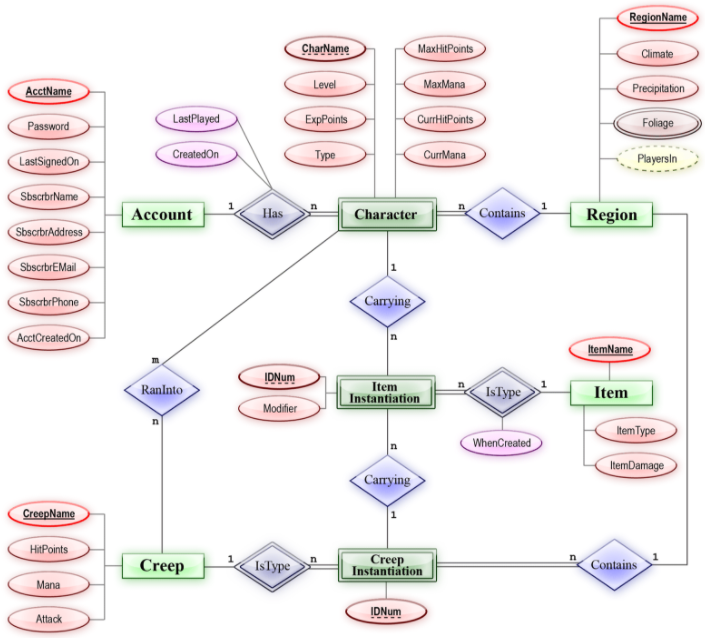
\includegraphics[width=\textwidth]{erChenNotation.png}
    \attribution{https://ru.wikipedia.org}
\end{center}

Прямоугольники означают сущности, овалы --- их свойства, ромбы --- связи между сущностями (которые сами могут иметь какие-то свойства). Связи могут иметь кратность (один к одному, один ко многим, даже многие ко многим), какой-то атрибут может быть назначен первичным ключом. Никогда не видел, чтобы эта нотация использовалась на практике.

Реально используются сейчас разные варианты нотации <<вороньей лапки>>:

\begin{center}
    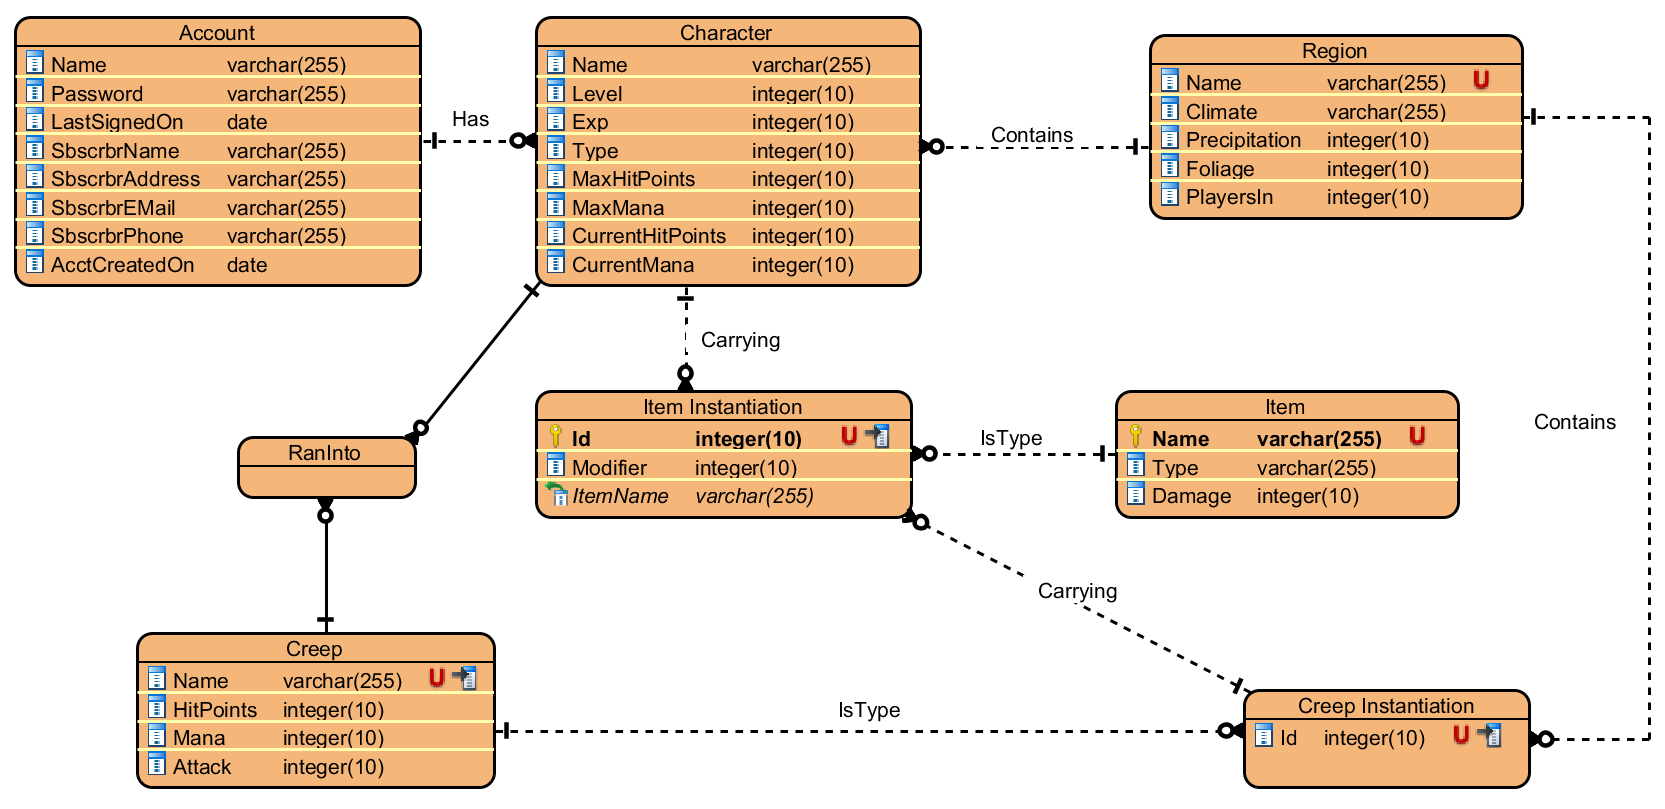
\includegraphics[width=\textwidth]{erCrowsFoot.png}
\end{center}

Нотация получила своё название за обозначение множественности связи (три разветвляющиеся линии на конце связи, похожие на птичью ногу). Её важное отличие от нотации Чена в том, что атрибуты в ней рисуются прямо внутри сущности, что делает диаграммы гораздо более компактными. Здесь тоже можно назначить один из атрибутов первичным ключом, задать ограничения уникальности и т.д., но детали нотации несколько различаются от инструмента к инструменту, поэтому не будем здесь на ней подробно останавливаться (благо такие диаграммы вы наверняка уже видели в контексте баз данных).

\section{Диаграммы конечных автоматов}

Диаграммы конечных автоматов (также известные как диаграммы состояний) --- это на самом деле несколько упрощённые диаграммы Харела, предложенные им ещё в 1987 году, которые попали в UML с минимальными изменениями. Это второй вид диаграмм UML, имеющий исполнимую семантику. Предназначены эти диаграммы для моделирования поведения <<реактивных>> систем (или частей системы), то есть систем, которые находятся в некоторых чётко определённых состояниях, от которых зависит их поведение, и могут реагировать на события, переходя из состояния в состояние и, возможно, делая при переходах полезную работу. Примеры реактивных систем --- это сетевое соединение (которое может быть открыто, закрыто, открываемо в данный момент, закрываемо, и в зависимости от этого передаёт или не передаёт пакеты), либо классический пример с торговым автоматом, с которого начинался рассказ про моделирование вообще.

Выглядят диаграммы конечных автоматов так:

\begin{center}
    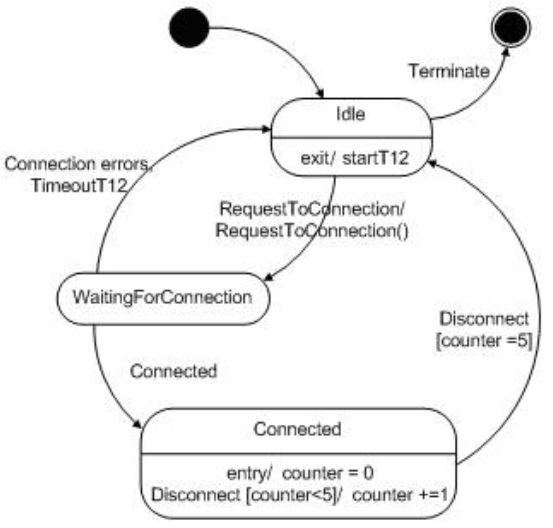
\includegraphics[width=0.4\textwidth]{stateTransitionExample.png}
\end{center}

Прямоугольниками со скруглёнными углами рисуются состояния, у состояния есть имя и (опционально) действия, выполняемые в состоянии (например, действие по выходу или внутренний переход по событию, как у Connected --- получив событие Disconnect, оно проверяет счётчик, и если счётчик меньше 5, он увеличивается на 1 и мы остаёмся в том же состоянии). Состояния связаны переходами, над переходом пишется событие, которое инициирует переход и, опционально, стражник (guard) (логическое условие, которое должно быть истинно, чтобы переход состоялся) и действие, выполняемое при переходе. События со стражниками должны быт взаимно исключающими, недетерминированные автоматы считаются некорректными. Есть псевдосостояния начала и конца, переход из псевдосостояния начала происходит мгновенно, переход в состояние конца заканчивает исполнение.

Внешне диаграммы конечных автоматов похожи на диаграммы активностей, но есть важные семантические различия:

\begin{itemize}
    \item На диаграмме активностей рисуются активности, система в них не задерживается, а сразу переходит дальше; на диаграмме конечных автоматов рисуются состояния --- стабильные отрезки жизненного цикла объекта, в которых он находится большую часть времени и может из них выйти только если что-то произойдёт;
    \item Полезная работа на диаграммах активностей производится в активностях, на диаграммах автоматов --- как правило, при переходе;
    \item Диаграммы активностей моделируют один метод объекта (или какую-то функцию или что-то такое), диаграммы конечных автоматов --- целый объект (состояния моделируются полями объекта).
\end{itemize}

Более подробно про синтаксис:

\begin{center}
    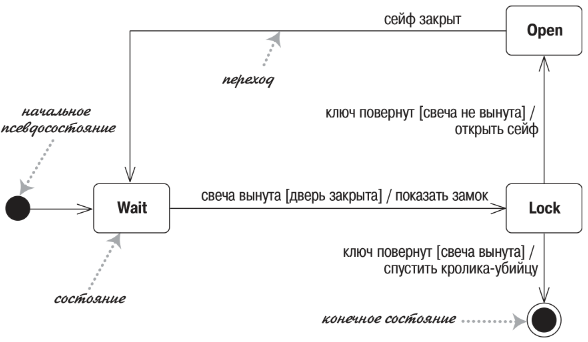
\includegraphics[width=0.7\textwidth]{stateTransitionSyntax.png}
    \attribution{М. Фаулер, UML. Основы}
\end{center}

Внутри состояния могут быть:

\begin{itemize}
    \item entry activity --- то, что делается при входе в состояния по любому из переходов;
    \item exit activity --- то, что делается при выходе из состояния по любому исходящему переходу (и входная, и выходная деятельность --- это, как правило, вызовы метода);
    \item do activity --- деятельность, выполняющаяся всегда, когда система находится в таком-то состоянии (например, попытки подключения к сети для мобильного телефона);
    \item внутренний переход --- переход по событию, который ведёт в то же состояние и не приводит к срабатыванию entry и exit activity. Переход вполне может быть полноценным переходом в то же состояние (рисуется как петля в графе), тогда entry и exit activity работают как обычно, хоть состояние и не меняется.
\end{itemize}

Событие, кстати, это нечто внешнее по отношению к системе, на что система может реагировать. Примеры событий --- действие пользователя, сетевой пакет, считывание символа (если речь идёт об автоматном лексическом анализаторе, который, кстати, хоть и несколько необычный, но тоже пример реактивной системы, которая прекрасно моделируется конечными автоматами).

Надпись на переходе имеет следующий синтаксис: \verb|[<trigger> [‘,’ <trigger>]* [‘[‘ <guard>’]’] [‘/’ <behavior-expression>]]| --- один переход может реагировать на несколько событий сразу, иметь опционального стражника (в квадратных скобках) и через слеш действие (вызов метода или отсылку к диаграмме активностей, которая поясняет, что нужно делать при переходе).

Есть вложенные состояния с переходами сразу из всех внутренних состояний:

\begin{center}
    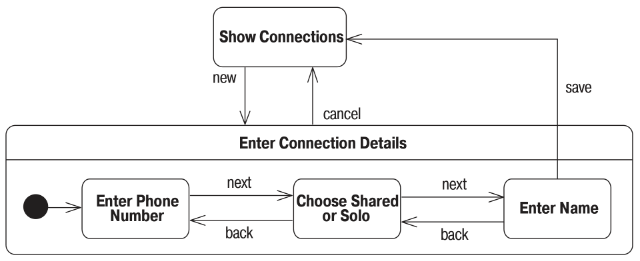
\includegraphics[width=0.7\textwidth]{stateTransitionNestedStates.png}
    \attribution{М. Фаулер, UML. Основы}
\end{center}

Тут состояние <<Enter connection details>> содержит внутри свой конечный автомат, который начинает работать со стартового псевдосостояния когда выполняется переход <<new>>. При этом переход <<save>> возможен только из состояния <<Enter Name>>, а вот переход <<cancel>> возможен из любого вложенного состояния (это замена нестандартному псевдосостоянию со звёздочкой из диаграммы выше).

Ещё бывают параллельные состояния и псевдосостояние истории:

\begin{center}
    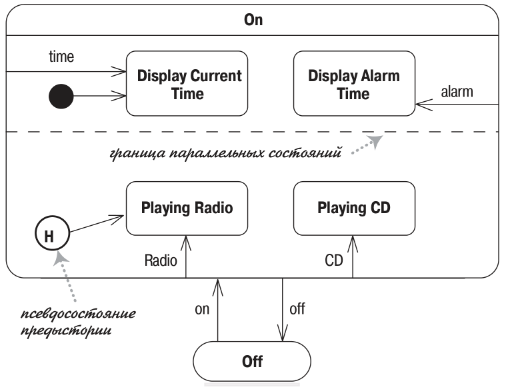
\includegraphics[width=0.6\textwidth]{stateTransitionParallelStates.png}
    \attribution{М. Фаулер, UML. Основы}
\end{center}

Это часы с радио и будильником. Проигрывание звука и время работают независимо, поэтому по сути это два автомата, работающих параллельно (что и показывает горизонтальная прерывистая линия, разделяющая параллельные подавтоматы). Стрелки от объемлющего состояния к вложенным означают, что система, находясь в объемлющем состоянии, реагирует на такие-то события и изменяет внутреннее состояние (например, часы по умолчанию показывают текущее время, но если пользователь нажал на кнопку <<будильник>>, начинает показывать время, на которое будильник установлен). Псевдосостояние истории запоминает последнее вложенное состояние, в котором находился автомат, и возвращает автомат в него. Например, часы по умолчанию включают радио, но если пользователь включил воспроизведение компакт-дисков (если кто помнит, что это такое) и выключил часы, то при следующем включении они снова будут проигрывать компакт-диски.

А вот так рисуются активности внутри состояния:

\begin{center}
    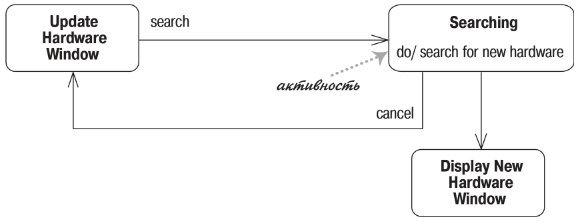
\includegraphics[width=0.6\textwidth]{stateTransitionInternalEventExample.png}
    \attribution{М. Фаулер, UML. Основы}
\end{center}

А вот так --- внутренние переходы и entry/exit-события:

\begin{center}
    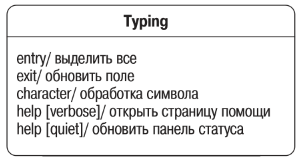
\includegraphics[width=0.35\textwidth]{stateTransitionInternalEvents.png}
    \attribution{М. Фаулер, UML. Основы}
\end{center}

Как видим, синтаксис очень похож на то, что пишется при переходе.

\subsection{Генерация кода}

Конечные автоматы хороши тем, что по ним можно легко и приятно генерировать код, в силу их стандартизованной семантики. Рассмотрим пример с кроликом-убийцей из книжки Фаулера:

\begin{center}
    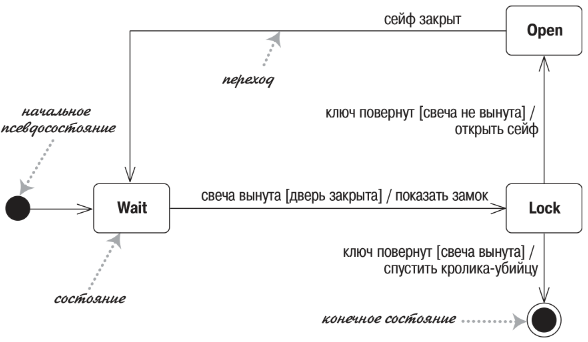
\includegraphics[width=0.8\textwidth]{stateTransitionSyntax.png}
    \attribution{М. Фаулер, UML. Основы}
\end{center}

Первый, самый простой способ сгенерировать код --- это сгенерировать гигантский switch, внутри которого чуть менее гигантские switch-и. Внешний switch --- по текущему состоянию автомата, внутренние --- по событиям, на которые находясь в данном состоянии автомат может реагировать. Внутри --- проверка условий стражников, выполнение действия по переходу и переход в следующее состояние. Состояние моделируется enum-ом, хранящимся как поле объекта. Для нашего примера получится что-то такое:

\begin{minted}{java}
public void handleEvent(PanelEvent anEvent) {
    switch (currentState) {
        case PanelState.Open:
            switch (anEvent) {
                case PanelEvent.SafeClosed:
                    currentState = PanelState.Wait;
            }
            break;
        case PanelState.Wait:
            switch (anEvent) {
                case PanelEvent.CandleRemoved:
                    if (isDoorOpen) {
                        revealLock();
                        currentState = PanelState.Lock;
                    }
            }
            break;
        case PanelState.Lock:
            switch (anEvent) {
                case PanelEvent.KeyTurned:
                    if (isCandleIn) {
                        openSafe();
                        currentState = PanelState.Open;
                    } else {
                        releaseKillerRabbit();
                        currentState = PanelState.Final;
                    }
            }
            break;
    }
}
\end{minted}

Это работает, но если этот код надо сопровождать, никто от него не будет в восторге. Для сколько-нибудь содержательных автоматов получается один метод на тысячи строк. Поэтому можно использовать таблицу состояний и универсальный интерпретатор, который просто ищет в таблице текущее состояние и событие, и выполняет то, что там написано. Вариантов таблиц состояний может быть много, но вот пример из книжки Фаулера:

\begin{center}
    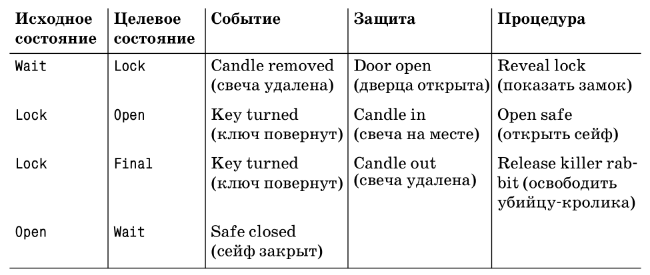
\includegraphics[width=0.6\textwidth]{stateTransitionStateTable.png}
    \attribution{М. Фаулер, UML. Основы}
\end{center}

Таблица состояний обычно либо хранится как файл данных рядом с программой, либо вкомпилируется в исходный код. 

Такой подход очень популярен в лексическом и синтаксическом анализе, но отлаживать или просто понимать такие программы очень тяжело. Поэтому есть ещё один, более объектно-ориентированный способ симулировать автомат: паттерн проектирования <<Состояние>>:

\begin{center}
    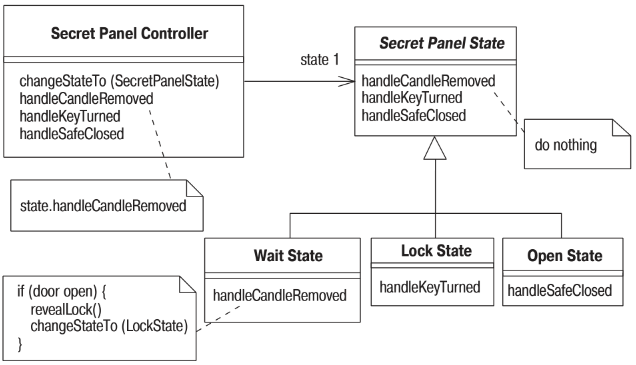
\includegraphics[width=0.6\textwidth]{stateTransitionStatePattern.png}
    \attribution{М. Фаулер, UML. Основы}
\end{center}

Автомат представляется в виде класса, который имеет в качестве поля ссылку на интерфейс <<текущее состояние>>. Этот интерфейс имеет столько методов, сколько всего разных событий может обрабатывать автомат. Интерфейс реализуют конкретные классы, отвечающие за конкретные состояния, они определяют те методы интерфейса, на которые могут реагировать, там уже проверяют условия стражников и выполняют действие при переходе. Каждый такой метод возвращает объект-состояние, в которое должен перейти автомат дальше. То есть, по сути, это тот же switch, где самый большой switch (по состояниям) спрятан в таблицу виртуальных методов. Такой подход делает реализацию автомата более-менее читаемой, ограничивает ответственность каждого класса только одним состоянием и позволяет очень легко добавить новые состояния, поэтому очень популярен при <<ручной>> реализации автоматов.

\section{Диаграммы последовательностей}

Следующий тип диаграмм UML, использующийся при моделировании поведения --- это диаграммы последовательностей (sequence diagrams). Они применяются для визуализации взаимодействия между объектами --- передачи сообщений, возврата значений, времени жизни объекта. Выглядят диаграммы следующим образом:

\begin{center}
    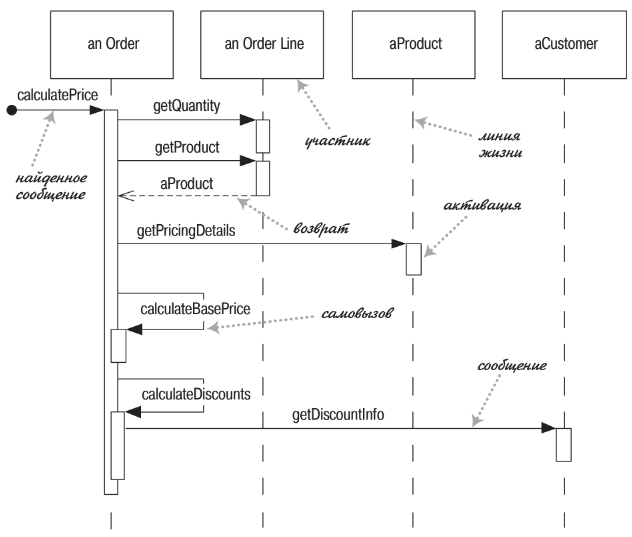
\includegraphics[width=0.8\textwidth]{sequenceDiagramSyntax.png}
    \attribution{М. Фаулер, UML. Основы}
\end{center}

На диаграмме рисуются объекты (обратите внимание, не классы), из каждого объекта выходит \textit{линия жизни} (пунктирная линия), на которой расположены \textit{линии активации} (длинный белый прямоугольник). Линия жизни показывает, когда объект вообще существует в памяти, линия активации --- когда объект занят какой-то работой (то есть работает либо его метод, либо метод, вызванный из его метода, или, более формально, какой-либо из методов объекта находится на стеке вызовов). Линий активации одновременно может быть несколько --- рекурсивные вызовы. Стрелки между линиями активации обозначают сообщения --- как правило, это вызовы методов, и поэтому они ведут в начало соответствующих вызванному методу линий активации. Обратите внимание, что стрелка не может выходить из неактивного объекта и не может входить <<в никуда>>.

Такая диаграмма позволяет разобраться в даже довольно сложных протоколах взаимодействия, поэтому применяется при многопоточном и асинхронном программировании, чтобы визуализировать общение между потоками/асинхронные вызовы. Также такие диаграммы очень популярны при описании телекоммуникационных протоколов (на самом деле, есть отдельный язык MSC (Message Sequence Charts), который применяется независимо от UML, но диаграммы последовательностей являются его почти копией).

Имеется и ряд менее очевидных применений: 

\begin{itemize}
    \item на этапе анализа предметной области для визуализации последовательности коммуникаций между участниками взаимодействия;
    \item на этапе проектирования для составления плана тестирования --- кто в каком порядке кого должен дёргать и кто когда чем должен отвечать;
    \item на этапе отладки, для визуализации логов работающей системы.
\end{itemize}

\section{Коммуникационные диаграммы}

Коммуникационные диаграммы --- это по сути те же диаграммы последовательностей, только <<с высоты птичьего полёта>>. Они так же применяются для визуализации взаимодействия между объектами, так же подходят только для визуализации одного сценария взаимодействия и так же показывают последовательность обмена сообщениями:

\begin{center}
    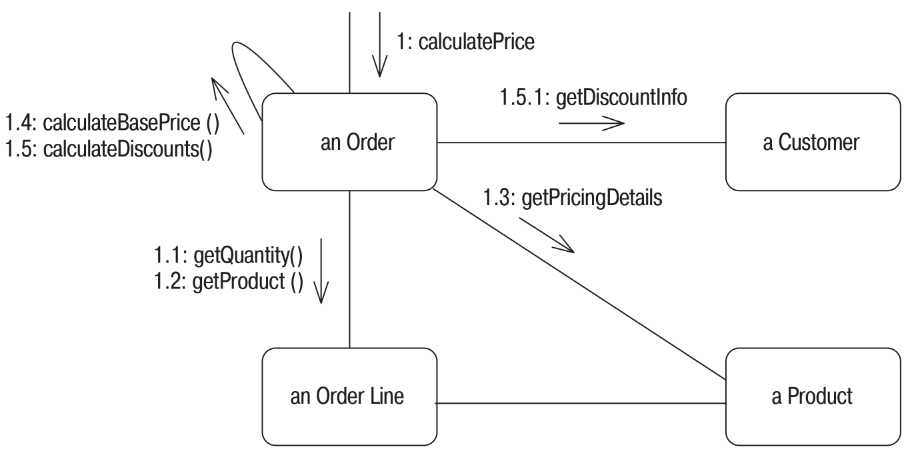
\includegraphics[width=0.6\textwidth]{communicationDiagram.png}
    \attribution{М. Фаулер, UML. Основы}
\end{center}

Однако на диаграммах последовательностей поведение объектов рисуется снизу вверх, то есть, условно, по оси X откладываются объекты, по оси Y --- время. На коммуникационных диаграммах объекты размещаются на двумерной плоскости, а порядок взаимодействия определяется числовыми индексами на стрелках. Это основное преимущество и основной недостаток таких диаграмм --- они гораздо компактнее диаграмм последовательностей, но порядок действий во времени на них не очевиден.

Вот более содержательный пример, диаграмма коммуникаций для онлайн-магазина книг:

\begin{center}
    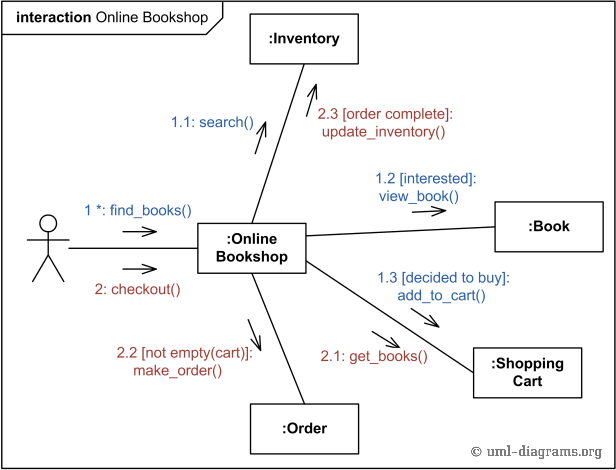
\includegraphics[width=0.6\textwidth]{communicationDiagramExample.png}
    \attribution{http://www.uml-diagrams.org/}
\end{center}

Сначала пользователь делает запрос find\_books(), который обрабатывается объектом типа Online Bookshop (до двоеточия пишется имя объекта, если оно важно, после --- имя типа, если оно важно). Вызов find\_books() приводит к вызову search(), view\_book() и add\_to\_cart() в именно такой последовательности. Обратите внимание на нумерацию запросов: 1.1 означает, что это первый вызов внутри вызова 1, 1.3 --- третий вызов внутри вызова 1. Дальше пользователь выполняет запрос checkout(), который обрабатывается с помощью ещё двух вызовов.

\section{Диаграммы составных структур}

Диаграммы составных структур предназначены больше для проектирования аппаратного обеспечения, которое состоит из стандартизованных блоков, соединённых стандартными интерфейсами. По сути, диаграммы представляют собой продвинутые диаграммы компонентов --- тут тоже рисуются крупные блоки, из которых состоит система, интерфейсы блоков, порты, связи. Однако же если диаграммы компонентов --- это диаграммы, показывающие структуру времени компиляции, то на диаграммах составных структур внутри объемлющей компоненты не другие компоненты, а \textit{роли}. Разница в том, что роль --- это что-то вроде объекта, на диаграмме может быть несколько ролей одного типа, которые по-разному связаны друг с другом и делают разную работу. Так же, как объекты, роли имеют тип. В работающей системе роль может играть любая компонента правильного типа. Вот небольшой пример диаграммы:

\begin{center}
    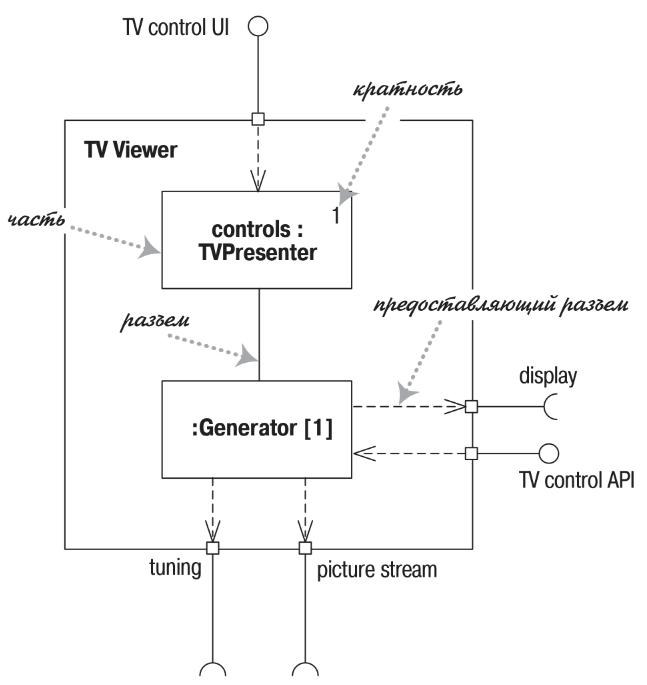
\includegraphics[width=0.5\textwidth]{compositeStructureDiagram.png}
    \attribution{М. Фаулер, UML. Основы}
\end{center}

Тут controls и :Generator --- это роли, в качестве controls может выступать любая компонента, реализующая интерфейс TVPresenter. \verb|[1]| --- это кратность компоненты (и TVPresenter, и Generator в системе только один). Порты, интерфейсы и связи тут в целом такие же, как на диаграмме компонентов (только что связи называются <<разъёмами>>).

\section{Диаграммы коопераций}

Диаграммы коопераций --- это что-то среднее между диаграммами объектов и диаграммами классов. Вместо классов и объектов на них рисуются \textit{роли} --- сущности, на место которых может быть подставлен настоящий объект. Диаграммы показывают взаимодействие ролей в рамках одного сценария использования, например:

\begin{center}
    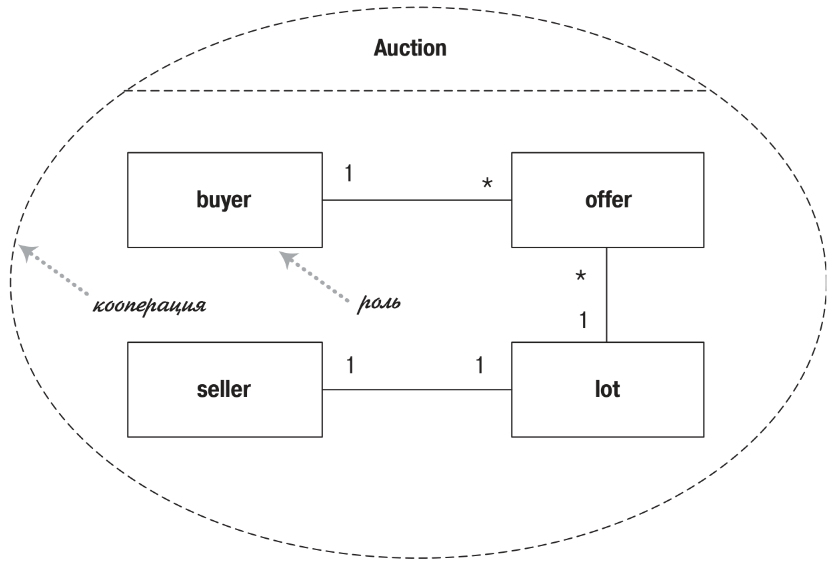
\includegraphics[width=0.7\textwidth]{cooperationDiagram.png}
    \attribution{М. Фаулер, UML. Основы}
\end{center}

Либо, что то же самое,

\begin{center}
    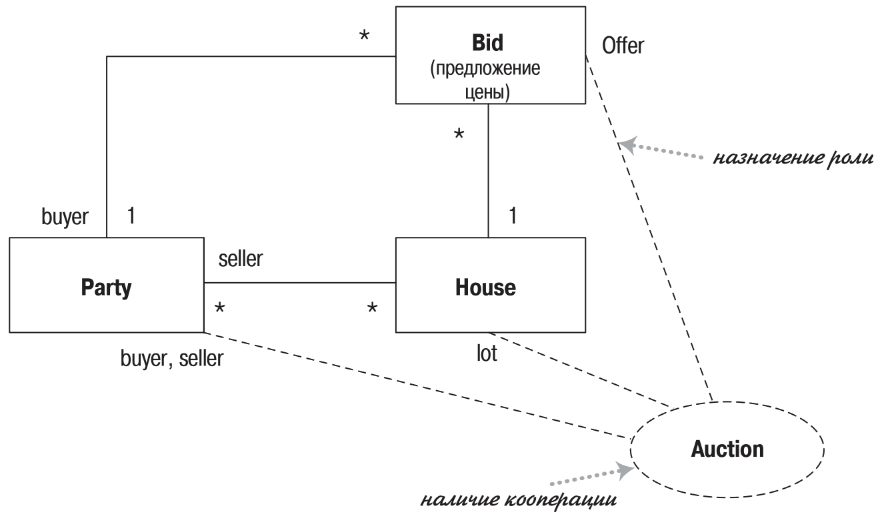
\includegraphics[width=0.7\textwidth]{cooperationAlternateNotation.png}
    \attribution{М. Фаулер, UML. Основы}
\end{center}

Здесь показана кооперация в рамках сценария использования <<Аукцион>>. Есть роли <<покупатель>>, <<продавец>>, которые могут взаимодействовать посредством лотов и предложений. Второй стиль рисования такой диаграммы больше похож на диаграмму классов, есть класс <<сторона>>, исполняющий роли <<покупатель>> и <<продавец>> в рамках данного взаимодействия.

Нужны такие диаграммы, чтобы проиллюстрировать конкретный сценарий использования системы, либо чтобы сосредоточиться на анализе конкретного сценария.

\section{Временные диаграммы}

Временные диаграммы создавались прежде всего для инженеров-электронщиков или для людей, проектирующих системы реального времени. Они нужны, чтобы визуализировать последовательности событий с чёткими временными ограничениями. Есть два варианта синтаксиса:

\begin{center}
    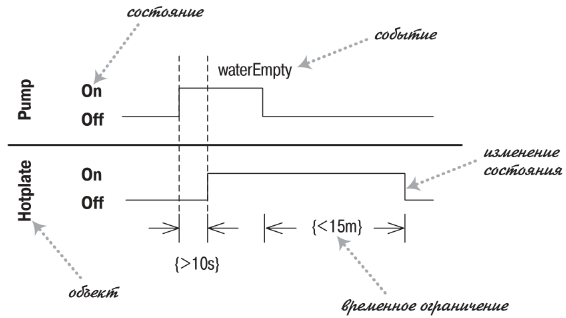
\includegraphics[width=0.6\textwidth]{timingDiagrams.png}
    \attribution{М. Фаулер, UML. Основы}
\end{center}

и

\begin{center}
    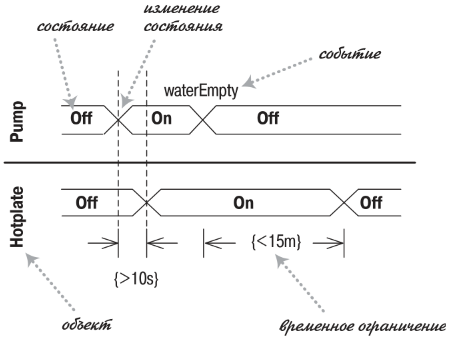
\includegraphics[width=0.6\textwidth]{timingDiagramsAlternate.png}
    \attribution{М. Фаулер, UML. Основы}
\end{center}

В обоих случаях рисуется временная шкала (время идёт слева направо), на ней вертикально располагаются объекты, которые могут находиться в некоторых состояниях. Первый вариант показывает переключение состояния как скачок линии, второй --- как пересечение линий с именем состояния внутри. Второй вариант удобнее, если состояний много, первый вариант нагляднее. Помимо состояний указываются и временные ограничения, в фигурных скобках, как принято в UML для ограничений.

Вот более солидный пример, для запроса браузера:

\begin{center}
    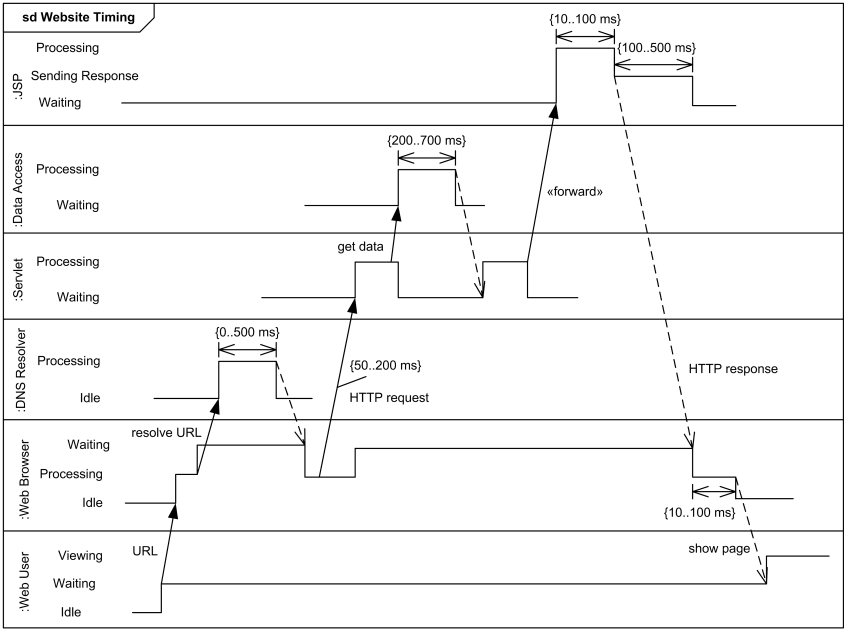
\includegraphics[width=0.9\textwidth]{timingDiagramExample.png}
    \attribution{http://www.uml-diagrams.org/}
\end{center}

Видно, что диаграмма позволяет отразить последовательность событий столь же наглядно, как диаграмма последовательностей, но ещё и наглядно показывает временные ограничения, и гораздо нагляднее в плане последовательности изменений внутреннего состояния объектов.

\section{Диаграммы обзора взаимодействия}

Диаграммы обзора взаимодействия --- это на самом деле не более чем совмещённые на одной диаграмме элементы диаграммы последовательностей и диаграммы активностей. Выглядят они так:

\begin{center}
    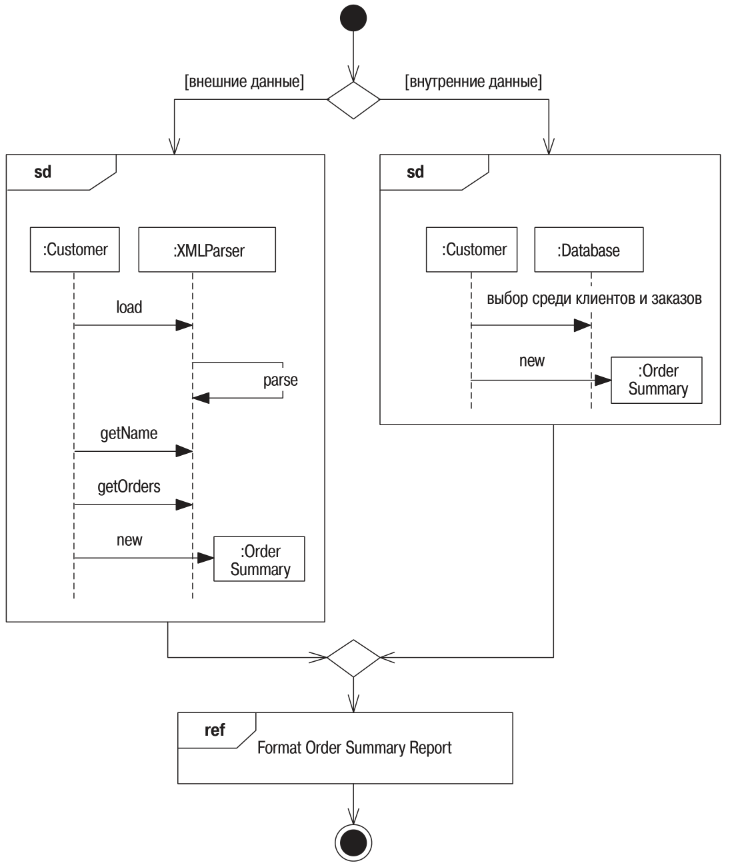
\includegraphics[width=0.7\textwidth]{interactionOverviewDiagrams.png}
    \attribution{М. Фаулер, UML. Основы}
\end{center}

Видно, что активность из диаграммы активностей может быть представлена в виде последовательности действий на диаграмме последовательностей. Применяются такие диаграммы, когда есть сложный алгоритм и нужна диаграмма последовательностей, которая бы его визуализировала, но имеется куча ветвлений и циклов. На диаграммах последовательностей есть фреймы, но для сколько-нибудь сложных алгоритмов они быстро сделают диаграмму нечитаемой --- тут-то диаграммы обзора взаимодействия и пригодятся. 

Вот более содержательный пример, валидация комментариев на сайте:

\begin{center}
    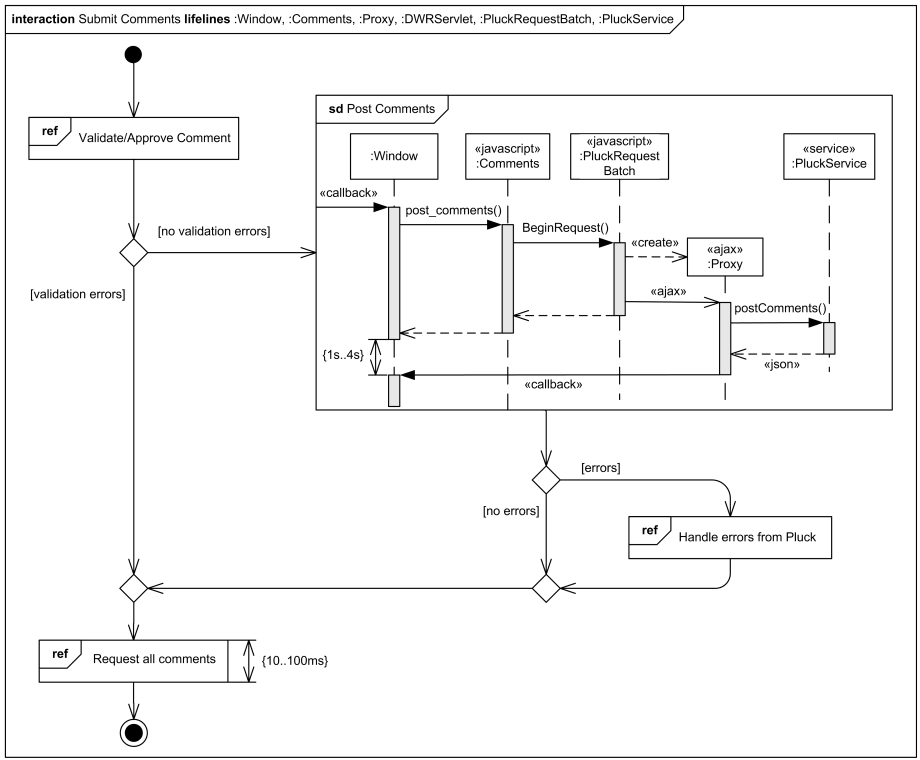
\includegraphics[width=0.9\textwidth]{interactionOverviewExample.png}
    \attribution{http://www.uml-diagrams.org/}
\end{center}

Как видно, на таких диаграммах тоже могут указываться временные ограничения.

\section{Диаграммы потоков данных}

На этом рассмотрение диаграмм UML закончилось. Но есть ещё полезные диаграммы, часто используемые сейчас при моделировании поведения программ, которые в UML не входят и даже не имеют там аналогов. 

Первая такая диаграмма, пожалуй, самая популярная и самая древняя из них --- это диаграмма потоков данных (Data Flow Diagram):

\begin{center}
    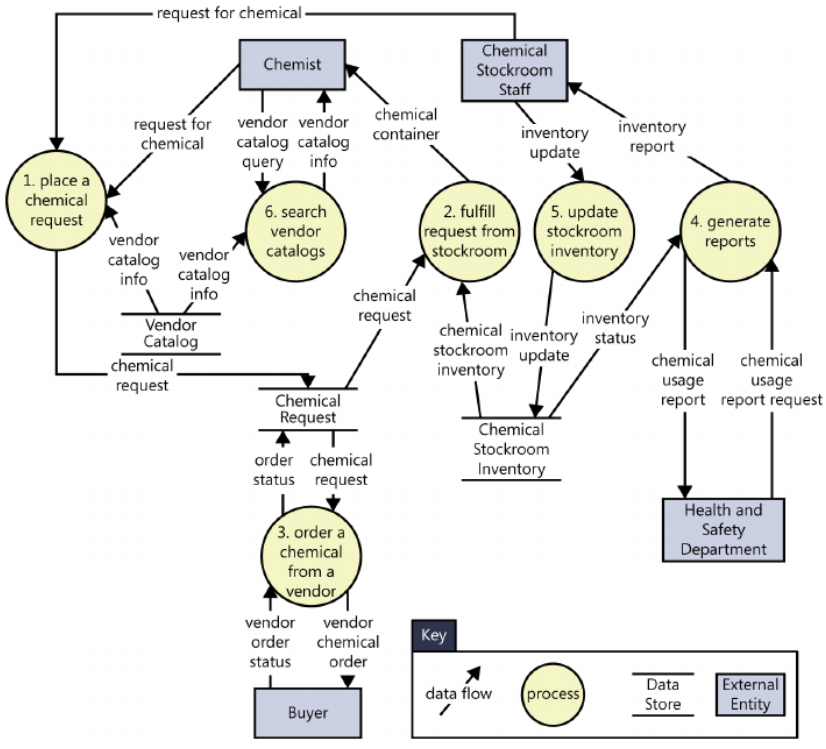
\includegraphics[width=0.8\textwidth]{dfd.png}
\end{center}

Синтаксис очень прост, есть один вид стрелок, который показывает поток данных, и три вида сущностей, между которыми, собственно, ходят данные:

\begin{itemize}
    \item процесс --- то, что может как-то преобразовывать данные внутри проектируемой системы, рисуется кружком;
    \item внешняя сущность --- то, что поставляет или потребляет данные, рисуется прямоугольником;
    \item хранилище --- то, где данные могут лежать, куда их можно поместить и забрать при необходимости, рисуется двумя горизонтальными линиями.
\end{itemize}

Такие диаграммы полезны как первый наборосок архитектуры системы (например, когда есть бизнес-процесс, где данные уже как-то ходят) или как иллюстрация к уже созданной системе. Потоки данных между функциональными блоками обычно интуитивно понятны и вместе с тем довольно сложны, так что диаграммы потоков данных могут сообщить много информации человеку, который начинает знакомиться с системой.

\section{Диаграммы IDEF0}

Диаграммы IDEF0 описывают декомпозицию системы и связи между её частями (которые, в свою очередь, тоже могут быть декомпозированы и раскрыты на отдельных диаграммах). Вот пример диаграммы IDEF0:

\begin{center}
    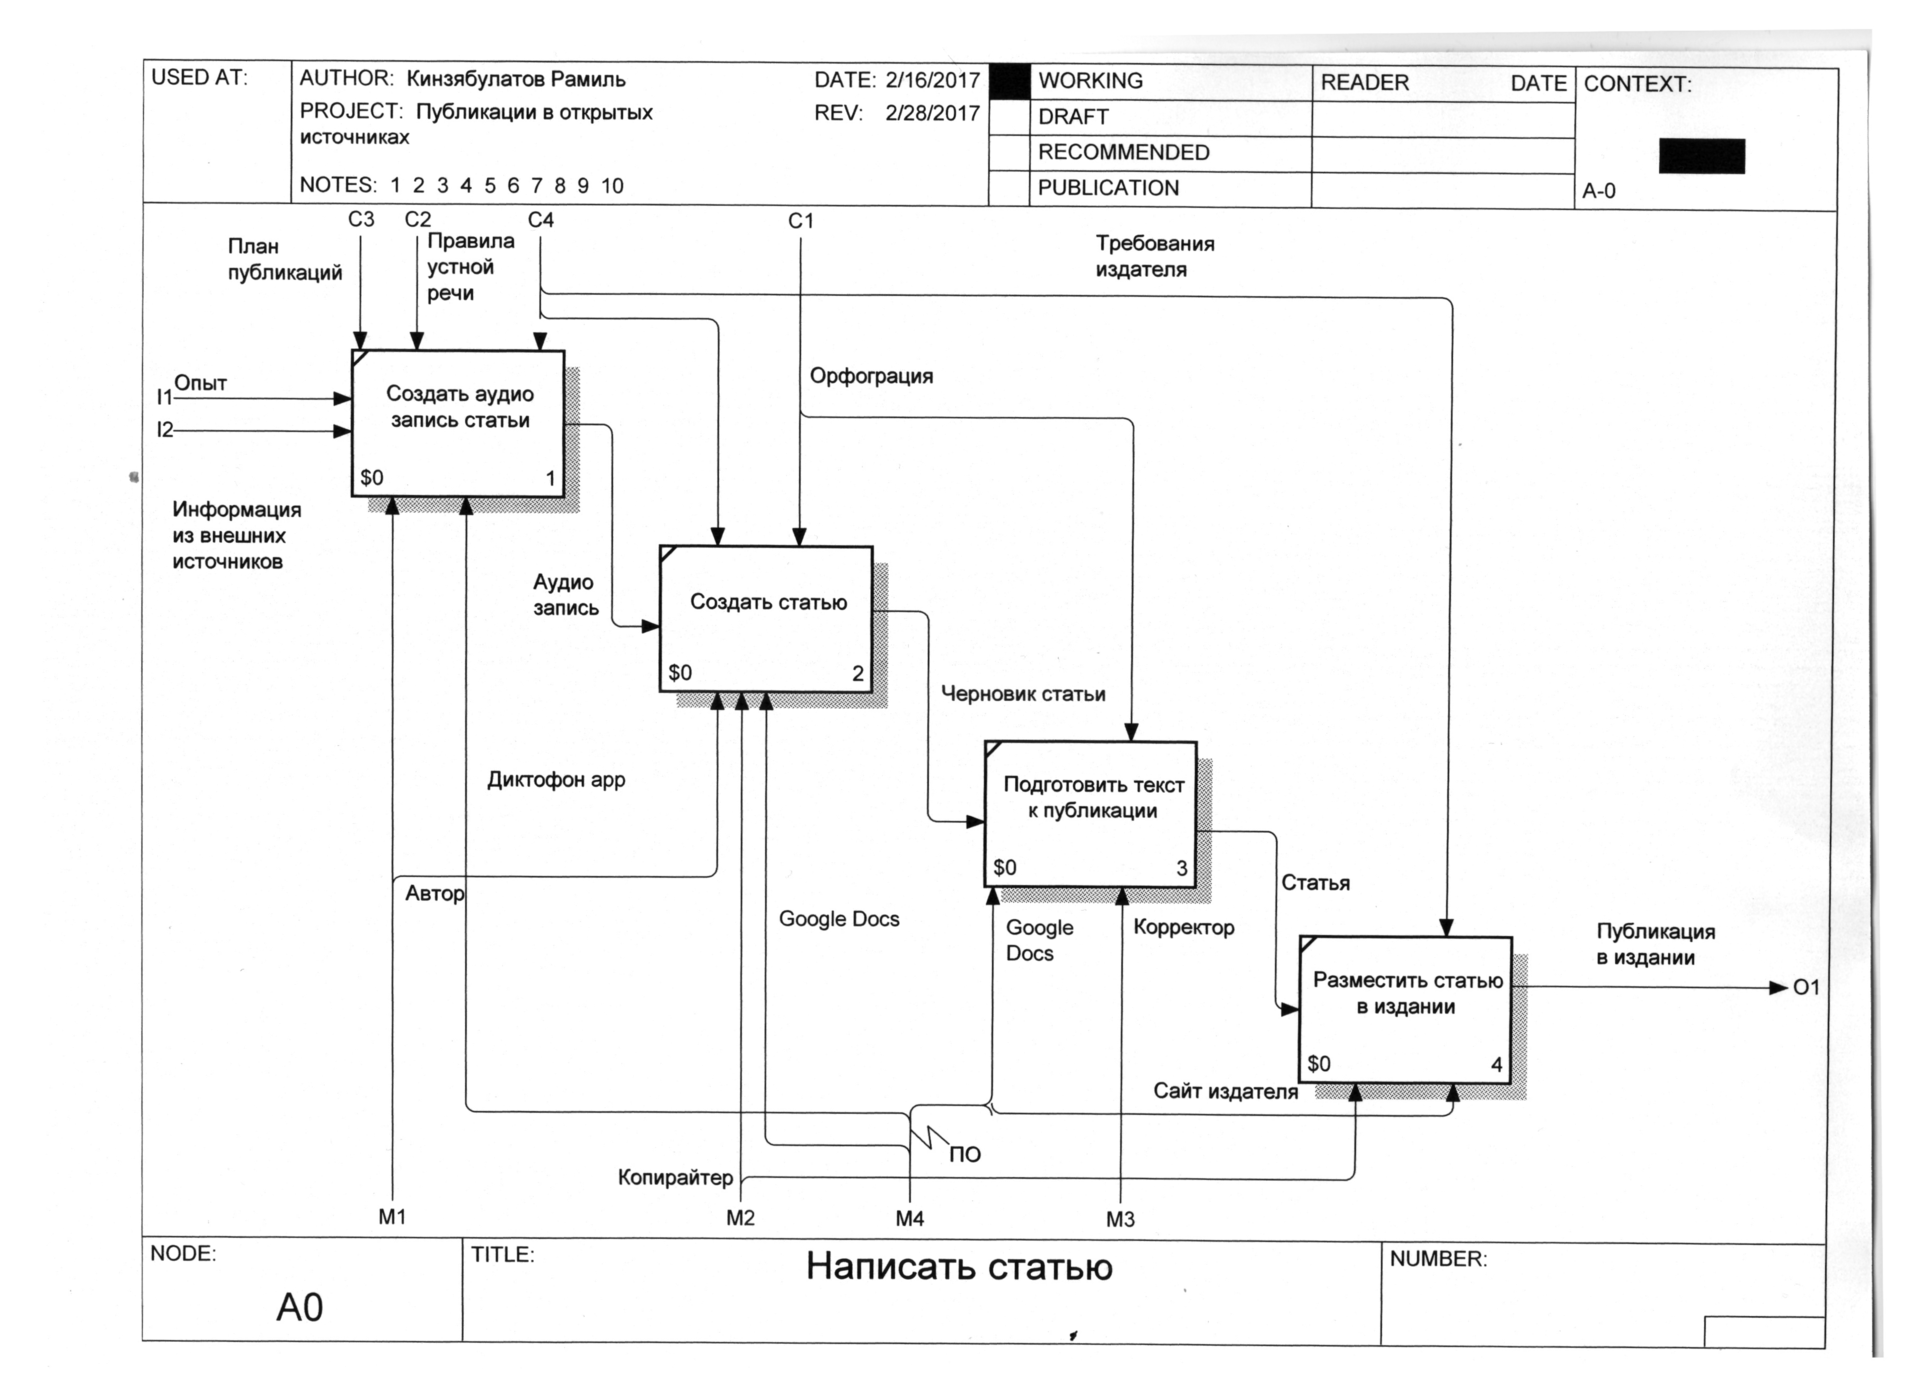
\includegraphics[width=\textwidth]{idef0.png}
    \attribution{https://habrahabr.ru/post/322832/}
\end{center}

Диаграмма состоит из блоков (у каждого из них есть имя и однозначно идентифицирующий его номер) и стрелок. Стрелки, входящие в блок слева --- материалы, которые блок перерабатывает в результаты (стрелки, выходящие справа). Сверху входят стрелки-управления --- то, что регламентирует работу блока и как-то управляет им. Снизу входят стрелки-механизмы (или ресурсы) --- это то, что блок непосредственно не перерабатывает, но необходимо блоку для работы. Например, блок может быть автозаводом, он перерабатывает запчасти в автомобили, как механизмы он использует станки и рабочих, как управление --- государственные и отраслевые стандарты, заказы от дилеров.

Над стрелками пишется, что из себя представляет эта стрелка, стрелки могут ветвиться (что может означать просто разделение ветки или детализацию --- тогда над отделившимися ветками пишутся уточнения надписи, которая была на исходной ветке) и сходиться в одну. Все ветки, входящие извне или исходящие с диаграммы, должны входить в блок или выходить из блока на диаграмме уровнем выше, и так далее до контекстной диаграммы. При этом используется однозначная схема именования стрелок.

Такие диаграммы чаще используются в анализе бизнес-процессов, в разработке собственно ПО чаще примменяются всё-таки диаграммы UML (диаграммы компонентов и диаграммы составных структур прекрасно заменяют IDEF0 в большинстве случаев). Тем не менее, аналитики IDEF0 любят и часто передают архитекторам как результаты своей работы, поэтому владеть IDEF0 архитекторам приходится.

\section{CASE-инструменты}

Ещё один немаловажный вопрос, который осталось обсудить --- это а где рисовать эти все диаграммы. Существуют специальные программы для визуального моделирования, которые отличаются от графических редакторов тем, что <<понимают>>, что в них рисуют (и позволяют рисовать, например, класс UML, а не просто прямоугольник с текстом), и умеют довольно многое делать с диаграммами --- генерировать код, интерпретировать диаграммы, строить диаграммы по коду, искать антипаттерны и т.д. Такие программы называются CASE-инструментами (от Computer-Aided Software Engineering).

Существующие CASE-инструменты можно условно разделить три категории.

\begin{itemize}
    \item <<рисовалки>> --- не очень умные инструменты, которые позволяют удобно рисовать диаграммы и иногда немного генерить по ним код, но не пытаются помогать с архитектурой или отладкой программы. Используются прежде всего как графические редакторы, специально заточенные под рисование диаграмм. Иногда люди увлекаются и начинают хотеть от них большего (например, генерации исполнимого кода по модели в Visio), но для этого есть лучшие альтернативы. Примеры таких инструментов:
    \begin{itemize}
        \item Microsoft Visio --- часть пакета Microsoft Office, на самом деле редактор диаграмм вообще, UML там один из десятков разных вариантов (от диаграмм из кружочков и стрелочек до планов помещений). Причём, UML, хоть и есть в стандартной поставке, там не очень продвинутый (некоторых элементов нотации не хватает), так что лучше отдельно поставить плагин с полноценной поддержкой UML (благо в Visio есть развитая плагинная система). Visio очень популярен в бизнес-среде, но платный (и, кажется, даже не входит в студенческую подписку СПбГУ, хотя и есть в компьютерных классах), и работает только под Windows.
        \item Dia --- Visio для Linux. Как часто бывает в Linux, бесплатна, с открытым исходным кодом, есть в репозитории любого уважающего себя дистрибутива, имеет кучу плагинов (в том числе, поддержку UML), умеет генерировать код. Больше практически ничего не умеет, поэтому как настоящая CASE-система не используется.
        \item SmartDraw --- рисовалка диаграмм вообще, не только программистских. Работает под Windows и имеет веб-версию, но платная.
        \item LucidChart --- примерно то же самое, несколько менее платное в том смысле, что сколько-то простых диаграмм на одного пользователя можно рисовать бесплатно. Имеет только веб-версию (и вроде как мобильные версии) и очень агрессивную рекламу.
        \item Creately --- простая, но относительно удобная веб-рисовалка. Рисует страшные как моя жизнь диаграммы, но если надо быстро что-то нарисовать без установки и длительного процесса регистрации, Creately вполне подойдёт.
    \end{itemize}
    \item Полноценные CASE-системы --- то самое, про что шла речь в предыдущем разделе. Как правило, платные, но, как правило, имеются бесплатные Community-версии, поэтому рекомендую пользоваться именно этими штуками, а не <<рисовалками>>. Как правило, все такие штуки десктопные, кроссплатформенные, с несколько урезанной браузерной версией. Популярные примеры:
    \begin{itemize}
        \item Enterprise Architect --- довольно популярный в IT-индустрии инструмент, более-менее всё умеет (не только UML, но и BPMN, SysML и другие полезные штуки) и не очень дорог (от 300\$ за лицензию и без бесплатной версии, так что для бедных студентов или инди-разработчиков так себе, но даже для средних стартапов это копейки).
        \item Rational Software Architect --- бывший Rational Rose (самый первый инструмент, поддерживавший UML), переписанный на платформе Eclipse. Тоже более-менее всё умеет, зато дороговат и опять-таки без бесплатной версии. Ни разу не видел, чтобы его использовали при практической разработке ПО, возможно это как-то связано с крайним неудобством его официального сайта. Достоин упоминания из-за отличной поддержки архитектурных рефакторингов.
        \item MagicDraw --- говорят, довольно хорошая и довольно популярная CASE-система, но, опять-таки, не видел её в деле.
        \item Visual Paradigm --- сам ей пользуюсь и встречал в индустрии, очень рекомендую. Умеет очень много чего, но основное её достоинство --- это usability. И наличие Community-версии.
        \item GenMyModel --- скорее, очень продвинутая браузерная <<рисовалка>>, чем настоящая CASE-система, но умеет генерировать код, умеет UML, BPMN и ещё некоторые нотации, имеет репозиторий, так что попала именно в эту категорию. В отличие от перечисленных выше настоящих CASE-систем, вообще не имеет десктопной версии, зато бесплатна для личного использования. Рекомендую как продвинутую замену Creately.
    \end{itemize}
    \item Прочие инструменты. Направлены в основном на быстрое иллюстрирование документации или веб-страниц чем-то, похожим на UML-диаграммы, позволяют текстом описать, что надо нарисовать. Наверное, будет приятно хардкорным кодерам, которые мышку в руках никогда не держали. Примеры (рекомендую покликать на ссылки, чтобы хотя бы знать, что так бывает):
    \begin{itemize}
        \item \url{https://www.websequencediagrams.com/} --- как намекает название, инструмент для рисования диаграмм последовательностей UML. Диаграммы описываются на очень простом текстовом языке, например, \verb|A->B: text| позволит нарисовать диаграмму с двумя объектами, один из которых шлёт другому сообщение <<text>>.
        \item \url{http://yuml.me/} --- генерирует по параметрам в URL картинки, которые можно вставлять на любую HTML-страницу. Например, \verb|<img src="http://yuml.me/diagram/scruffy/class/[Customer]->[Billing Address]" >| вставит диаграмму классов с двумя классами и ассоциацией между ними.
        \item \url{http://plantuml.com/} --- генерирует картинки (и даже ASCII-арт) по текстовому описанию. Например, \verb&Class01 <|-- Class02& сгенерирует диаграмму классов с двумя классами, один наследник другого. Не так удобно эти картинки куда-либо встраивать, зато может рисовать практически любые UML-диаграммы, и даже очень сложные, с десятками классов и кучей разных связей.
    \end{itemize}
\end{itemize}

\section{Литература}

\noindent\begin{minipage}{\textwidth}
    \begin{minipage}[c][6cm][c]{\dimexpr0.7\textwidth-0.5\Colsep\relax}
        На этом заканчивается обзор языков визуального моделирования. Для закрепления знаний очень рекомендую книжку М. Фаулер, UML. Основы. Краткое руководство по стандартному языку объектного моделирования. СПб., Символ-Плюс, 2011. 192 С. Книжка короткая, состоит в основном из картинок, но содержит, в целом, все знания, которые нужны, чтобы использовать на практике UML-диаграммы.
    \end{minipage}\hfill
    \begin{minipage}[c][6cm][c]{\dimexpr0.3\textwidth-0.5\Colsep\relax}
        
\includegraphics[width=0.6\textwidth]{umlBookCover.png}
    \end{minipage}%
\end{minipage}

\end{document}
